\documentclass{article}

\usepackage[scale=0.75,a4paper]{geometry}
\usepackage[utf8]{inputenc}
\usepackage[british]{babel}
\usepackage{csquotes}
\usepackage{graphicx}
\usepackage{subcaption}
\usepackage{float}
\usepackage{amsmath}
% \usepackage{amssymb}
\usepackage[separate-uncertainty=true]{siunitx}
\usepackage{physics}
\usepackage{minted}
\usepackage{titling}
% \usepackage{lipsum}
\usepackage[
    backend=biber,
    style=numeric
]{biblatex}

\addbibresource{references.bib}

% ====== table cosmetics ======
% \renewcommand{\arraystretch}{1.3}
% \setlength{\tabcolsep}{18pt}

% ====== shortcuts ======
\newcommand{\R}[1]{\mathrm{#1}}
\newcommand{\eps}{\varepsilon}
\newcommand{\ph}{\varphi}
\newcommand{\CC}{{C\nolinebreak[4]\hspace{-.05em}\raisebox{.3ex}{\scriptsize\bf ++}}}

% ====== style the title ======
\setlength{\droptitle}{-25pt}
\pretitle{\begin{center} \LARGE}
\posttitle{\end{center}}
\preauthor{}
\postauthor{}
\predate{\begin{center} \large }
\postdate{\end{center}}

% === Minted ===
\setminted{breaklines,linenos}

\begin{document}
\title{Optics with Imperfect Mirrors\\Part II Computational Project}
\author{}
\date{\today}
\maketitle

\abstract{
A computational study of the effects of deformations in the surface of telescope mirrors is performed. The far-field diffraction pattern of mirrors is computed in a \CC{} program using discrete Fourier transforms. The depth of the defects causes a decrease in the central intensity of the diffraction pattern, thus raising the lower bound on the brightness of observable objects. The central amplitude follows: $\psi_0 \propto \exp(-(\sigma_\eps/\lambda)^2 / 2\sigma_\psi^2)$, where $\sigma_\eps$ quantifies the typical defect depth. The spatial distribution of defects affects resolution, with smaller and denser deformations causing more spread-out fluctuations in the image.
}

\noindent\rule{0.85\textwidth}{0.4pt}


\section{Introduction}~\label{sec:intro}
Modern telescopes use very finely polished curved mirrors to create sharp images. However, errors are an inherent property of any physical system and any manufacturing process. Thus, regardless of the way mirrors are manufactured (e.g.\ spin-casting or polishing), there are still imperfections in their shape.

The aim of this paper is a computational investigation of the effects of imperfections in the shape of a telescope mirror on the image. Several relationships are studied, as suggested in the projects manual~\cite{manual}:
\begin{itemize}
    \item the effects of tapered illumination on the size and central intensity of the image.
    \item the effect of a central hole in the mirror, due to the secondary mirror.
    \item the effects of random and correlated phase errors, due to physical dents in the surface of the mirror. The dents cause phase errors due to the change in path length with respect to the smooth shape.
\end{itemize}

A more detailed analysis of the theory and techniques used is given in Section~\ref{sec:analysis}. Implementation details are discussed in Section~\ref{sec:impl}, and results are presented and discussed in Section~\ref{sec:res}.


\section{Analysis}~\label{sec:analysis}
In the analysis of this problem, we treat the far-field diffraction pattern of the mirror under uniform or Gaussian illumination. In the far field regime, the diffraction pattern of an aperture is given by the Fourier Transform of the aperture function \( A(x,y) \)~\cite[Chapter 10.2]{hecht}. This is a reasonable approximation as long as:
\begin{equation}\label{eqn:fraunhofer}
    \frac{R^2}{\lambda D} \ll 1,
\end{equation}
known as the Fraunhofer limit, where $R$ is the maximum extent of the aperture, $\lambda$ is the wavelength of radiation and $D$ is the distance from the aperture to the screen onto which the image is projected. In this problem we use:
\begin{align*}
    \lambda &= \SI{1}{mm} \\
    R &= \SI{6}{m},
\end{align*}
which would require a distance on the order of \SI{1}{km} for the far-field limit to hold. 

However, considering parabolic mirrors brings the image plane closer. Besides, we can work in angular coordinates, with the image space spanned by:
\begin{align*}
    p &= k \sin{\theta} \approx \frac{k x'}{D} \\
    q &= k \sin{\chi} \approx \frac{k y'}{D},
\end{align*}
where $x'$ and $y'$ are distances that would span a physical image plane, and $k$ is the wavenumber. We thus eliminate the dependence on $D$. In these coordinates, the diffraction pattern is:
\begin{equation}\label{eqn:diff}
    \psi(p, q) \propto \iint A(x, y) \exp \left( ipx + iqy \right) dx dy,
\end{equation}
which is just a Fourier transform of $A$. The dimensions of the diffraction pattern will always be given in terms of $p$ and $q$, and thus have units of \si{\per\metre}.

NB: Seemingly we've also eliminated the dependence on $\lambda$, but that will be needed again in the analysis of dented mirrors (Section~\ref{sec:analysis:bent}).

What is the meaning of this diffraction pattern? Since the incoming light is multiplied by the telescope's aperture function, the resulting image is a convolution of the astronomical objects being observed and the diffraction pattern of $A(x, y)$. Intuitively, for point-like stars, they will be seen through the telescope as ``copies'' of the diffraction pattern. Two factors are thus crucial:
\begin{itemize}
    \item The width of the central disk, which limits the resolution of the telescope. If two objects are closer than this central width, they cannot be resolved~\cite[Section~10.2.6]{hecht}.
    \item The central intensity, which sets a lower bound on the brightness of objects that can be observed.
\end{itemize}

\subsection{Discrete Fourier Transforms}\label{sec:analysis:dft}
The fact that the image is a Fourier transform of the aperture function is very useful. Fast Fourier Transform algorithms can compute discrete Fourier transforms of multi-dimensional data efficiently, and there exist many library implementations thereof. Here, the \CC{} \texttt{FFTW 3} library~\cite{fftw} was chosen, as suggested in the projects manual~\cite{manual}. It is a well-established and well-tested library with very good computational efficiency.

Minor adaptations are required to use the DFT algorithms in the library. The 1D discrete Fourier transform is defined as~\cite[Chapter 12.1]{NumRecipes}:
\begin{equation}
    H_k \propto \sum_{n=0}^{N-1} h_n\ \exp( 2\pi{}i \frac{kn}{N} ),
\end{equation}
with the corresponding frequency values:
\begin{equation}\label{eqn:fk}
    f_k = \frac{k}{N \Delta},\quad k = 0..N-1,
\end{equation}
where $\Delta$ is the sampling interval of the original signal. Comparing to a 1D discrete form of the diffraction integral (Equation~\ref{eqn:diff}):
\begin{equation}
    \psi_k \propto \sum_{n=0}^{N-1} A_n \exp( i p_k x_n ), \qq{where} x_n = n \Delta
\end{equation}
we see that we need to rescale:
\begin{equation}
    p_k = 2\pi f_k.
\end{equation}

\subsection{Testing}\label{sec:analysis:test}
To determine whether the program is outputting something sensible, we need to test it on a range of known results. Diffraction patterns for the following kinds of apertures are easy to compute analytically, and thus can be used for testing the program.

\paragraph{Rectangular aperture} A rectangular aperture of size $-a < x < a$, $-b < y < b$ has diffraction pattern:
\begin{equation}
    \psi(p, q) \propto \frac{\sin{\left( pa \right)}}{pa} \frac{\sin{\left( qb \right)}}{qb},
\end{equation}
thus it's expected to have the first zeros at:
\begin{equation}\label{eqn:test_rect}
    p = \pm \frac{\pi}{a} \qq{and} q = \pm \frac{\pi}{b}.
\end{equation}

\paragraph{Circular aperture} A circular aperture of radius $R$ has a diffraction pattern called an Airy disc, with angular radius:
\begin{equation}\label{eqn:test_circ}
    \sin{\theta} \approx 1.22 \frac{\lambda}{2R} \quad \Rightarrow \quad p = 1.22 \frac{\pi}{R}.
\end{equation}

Both of these minima should appear in the diffraction patterns, and the scaling with the inverse of the aperture size should be observable.

\subsection{Tapered aperture function}\label{sec:analysis:taper}
The amplitude of light illuminating a telescope mirror is often not uniform. A ``taper'' or ``grading'' is chosen, usually in the form of a Gaussian curve~\cite[Section~6.4]{RadioAstro}:
\begin{equation}
    A(r) = \begin{cases}
        e ^ {-r^2 / {2 \sigma^2}} &, r \leq R\\
        0 &, r > R
    \end{cases}, \qq{where} r^2 = x^2 + y^2.
\end{equation}

This is the multiplication of a Gaussian with a circular aperture of radius $R$. From the convolution theorem, its diffraction pattern is the convolution between another Gaussian and a Bessel function. Intuitively, this should lead to a ``smearing'' of the central maximum relative to a uniformly-lit mirror. Since the variance of a Gaussian is inversely proportional to the variance of its F.T., the smearing will be stronger at small $\sigma$.

Therefore, at small $\sigma$, the full width at half power (FWHP) should follow:
\begin{equation}
    \Delta p_{\R{hp}} \propto \sigma^{-1}.
\end{equation}
At large $\sigma$, as $A$ approaches uniform illumination, the image tends to a Bessel function, and the FWHP will approach a constant value. Besides, since at smaller $\sigma$ the integral of $|A|$ over the aperture is smaller, the central intensity should be smaller, tending to 0 as $\sigma \rightarrow 0$.

While the taper widens the central maximum, it also leads to suppression of the side lobes of the Airy pattern, thus possibly improving the resolution. See~\cite[Section~11.3]{hecht} for an explanation.

\subsection{Central hole}\label{sec:analysis:hole}
Classical telescopes, such as the Cassegrain design, have a central hole in the primary mirror due to the secondary mirror~\cite[Section~7.2.3]{RadioAstro}. The resulting aperture function can be viewed as the difference between that of the complete mirror $(A_{\R{complete}})$ and that of the hole $(A_{\R{hole}})$. Due to the linearity of the Fourier Transform, the diffraction pattern of this mirror should be the difference between the patterns of $A_{\R{complete}}$ and $A_{\R{hole}}$.

We can quantify how similar these results are by subtracting the image produced by a holed aperture from the difference of the images produced by $A_{\R{complete}}$ and $A_{\R{hole}}$.

Due to the Airy disc of the smaller $A_{\R{hole}}$ being larger than that of the complete mirror, we expect the entire central disc to be dimmer due to the hole. The secondary rings should become irregular, because they have different frequencies in the patterns of $A_{\R{complete}}$ and $A_{\R{hole}}$.

\subsection{Bent mirrors}\label{sec:analysis:bent}
\begin{figure}
    \centering
    \begin{minipage}{0.5\textwidth}
        \centering
        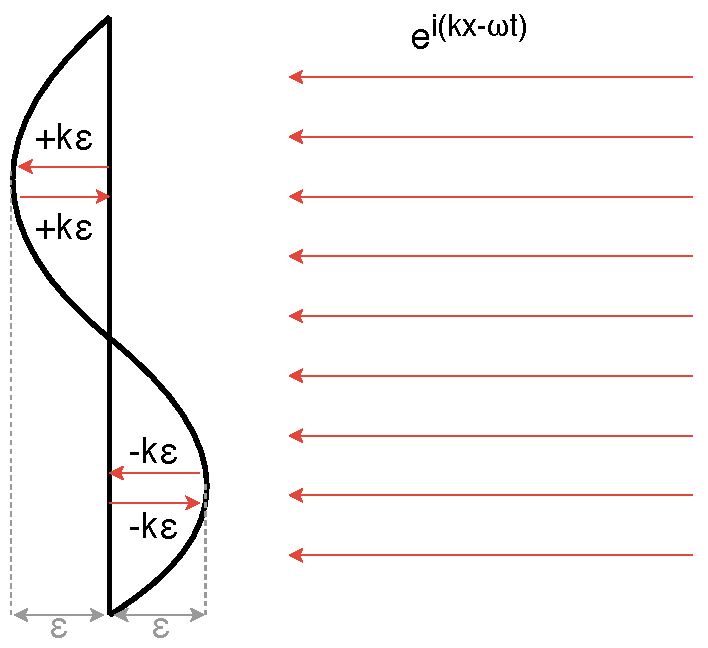
\includegraphics[width=0.7\textwidth]{pictures/mirror_dent.pdf}
    \end{minipage}%
    \hfill
    \begin{minipage}{0.4\textwidth}
        \caption{effect of deformations in the mirror surface on the phase of the wave. A deformation of depth $\eps$ produces an optical path difference of $2\eps$, one for the incident wave and one for the reflected wave.}\label{fig:bend}
    \end{minipage}
\end{figure}

Mirror surfaces could have deformations in them due to manufacturing errors, altering the phase of light. As seen in Figure~\ref{fig:bend}, the effect is that, for a dent of depth $\eps$, there is a path difference of $2\eps$, leading to a phase difference of:
\begin{equation}
    \Delta\ph = 2k\eps = \frac{4\pi}{\lambda}\eps
\end{equation}

We are going to investigate the effect of two types of phase errors:
\begin{itemize}
    \item without spatial correlation, with a given RMS $\sigma_\eps$
    \item spatially correlated on length $l_c$, to simulate deformations in the mirror.
\end{itemize}

The expected effect of these errors is to decrease the central intensity of the image, as they introduce decoherence to the light. We can also expect that errors on smaller correlation lengths will cause a wider spread of fluctuations in the beam pattern.

\section{Implementation}\label{sec:impl}
More complete implementation details and instructions are found in the file \texttt{readme.md}. This section discusses details that are critical to the performance of the program.

The overall logic flow of the program is:
The executable is invoked with one argument, naming a ``configuration file''. The instructions therein are read and executed in order, thus computing diffraction patterns for the described apertures. The results are printed to disk, and figures can then be produced by invoking the respective Python scripts for each problem.

\CC{} source files are in \texttt{src/cpp}, and plotting scripts in \texttt{src/scripts}. Sample configuration files can be found in \texttt{config}.

Note that, besides \texttt{FFTW}, I also used the GNU Scientific Library~\cite{gsl}, mainly for random number generators and statistics.

\subsection{Describing Apertures and Images}
In the \texttt{FFTW} library two-dimensional $N_x$ by $N_y$ arrays are represented as one-dimensional arrays of complex numbers (the inbuilt \texttt{complex} type~\cite{cppcomplex}) of length $N_x \times N_y$~\cite[Section 3.2]{fftw}.

Because working directly with a 1D representation of 2D data can be clunky, I decided to wrap this functionality in a class called \texttt{Array2d}, declared in the header with the same name. The class stores the data internally in the 1D array representation, but has a more user-friendly interface. It defines the \texttt{[i][j]} and \texttt{(i, j)} operators for easy access to the element in the $i^{th}$ row and $j^{th}$ column.

\paragraph{Memory allocation} One special feature of this class that breaks with convention is that the (compiler generated) copy constructor only performs a shallow copy, copying the pointer to the data array, but not the data itself. Only the explicitly defined constructor \mintinline{C++}{Array2d::Array2d(int nx, int ny)} uses \texttt{fftw\_alloc\_complex} to allocate new memory for the array. This means that the user of the class has finer control over where memory is allocated, which is important in the case of large arrays. For example, using IEEE double-precision floating point, which occupies 64 bits of memory, a $2^{13} \times 2^{13}$ array of complex numbers occupies around \SI{1}{GB} of memory.

For better understanding of when memory is allocated, compile the code with the variable \texttt{DEBUG\_OUT} set to \texttt{true} in \texttt{array2d.cpp}. Then the calls to the constructor and destructor of \texttt{Array2d} will be printed to console.

\paragraph{Aperture generators} These are a type of function that initialise an \texttt{Array2d} with a particular kind of aperture with given parameters. For example, there is a generator for circular apertures, one for circular Gaussian-illuminated, one for circular with random errors, etc.

\subsection{Configuration Files}
Configuration files are stored by convention in the \texttt{config} directory, and are a series of \texttt{key = value} lines. They contain:
\begin{itemize}
    \item \texttt{nx} and \texttt{ny}. These are the size of input and output arrays.
    \item \texttt{tasks}, what actions to perform on each of the shapes
    \item \texttt{n\_shapes}, the number of shapes
    \item for each shape, its properties: \texttt{type} (the name of the aperture generator), \texttt{lx} and \texttt{ly} (the domain of $A(x,y)$), and \texttt{params}, a list of parameters of the shape, e.g.\ the dimensions or the taper of Gaussian illumination.
\end{itemize}

\subsection{Parallelization}
The program can use multiple threads to process several shapes in parallel. The variable \texttt{N\_WORKERS} in \texttt{main.cpp} controls the number of threads (``workers'') used. Care must be taken to not run out of memory, as each thread allocates between 2 and 4 \texttt{Array2d} objects. The \texttt{FFTW} library only allows the creation of one Fourier transform plan at a time~\cite[Section 5]{fftw}. This means that a larger number of threads has a larger initialization time, since each worker thread creates its own plans.

\subsection{The \texttt{fftshift} operation}
The result of this operation is shifting the zero-frequency component of the spectrum from the beginning to the middle of an array. This takes advantage of the fact that the Fourier frequencies (Equation~\ref{eqn:fk}) are cyclic with period $1/\Delta$~\cite[Section~12.1.2]{NumRecipes}. Applying this is required to see a diffraction pattern as it would appear on a screen.

\subsection{Correlating errors}
As mentioned in Section~\ref{sec:analysis:bent}, we want to investigate the effects of spatially-correlated phase errors. To produce such deformations, we convolve random gaussian-distributed numbers with a gaussian shape of the desired correlation width, as suggested in the manual~\cite{manual}. Taking advantage of the convolution theorem, this is equivalent to multiplication of FTs of the two shapes, followed by a reverse FT. The numbers are then normalised to the desired RMS and set as the phase in the ``mirror'' array. The \texttt{corr\_errors} aperture generator implements this.

We want to ensure that the phase error produced by this method is the desired one, and that it doesn't change with the correlation length $l_c$. These properties are tested in Section~\ref{sec:res:rms}.

\section{Results and Discussion}\label{sec:res}
\subsection{Tests}

\begin{figure}
    \centering
    \begin{subfigure}{0.5\textwidth}
        \centering
        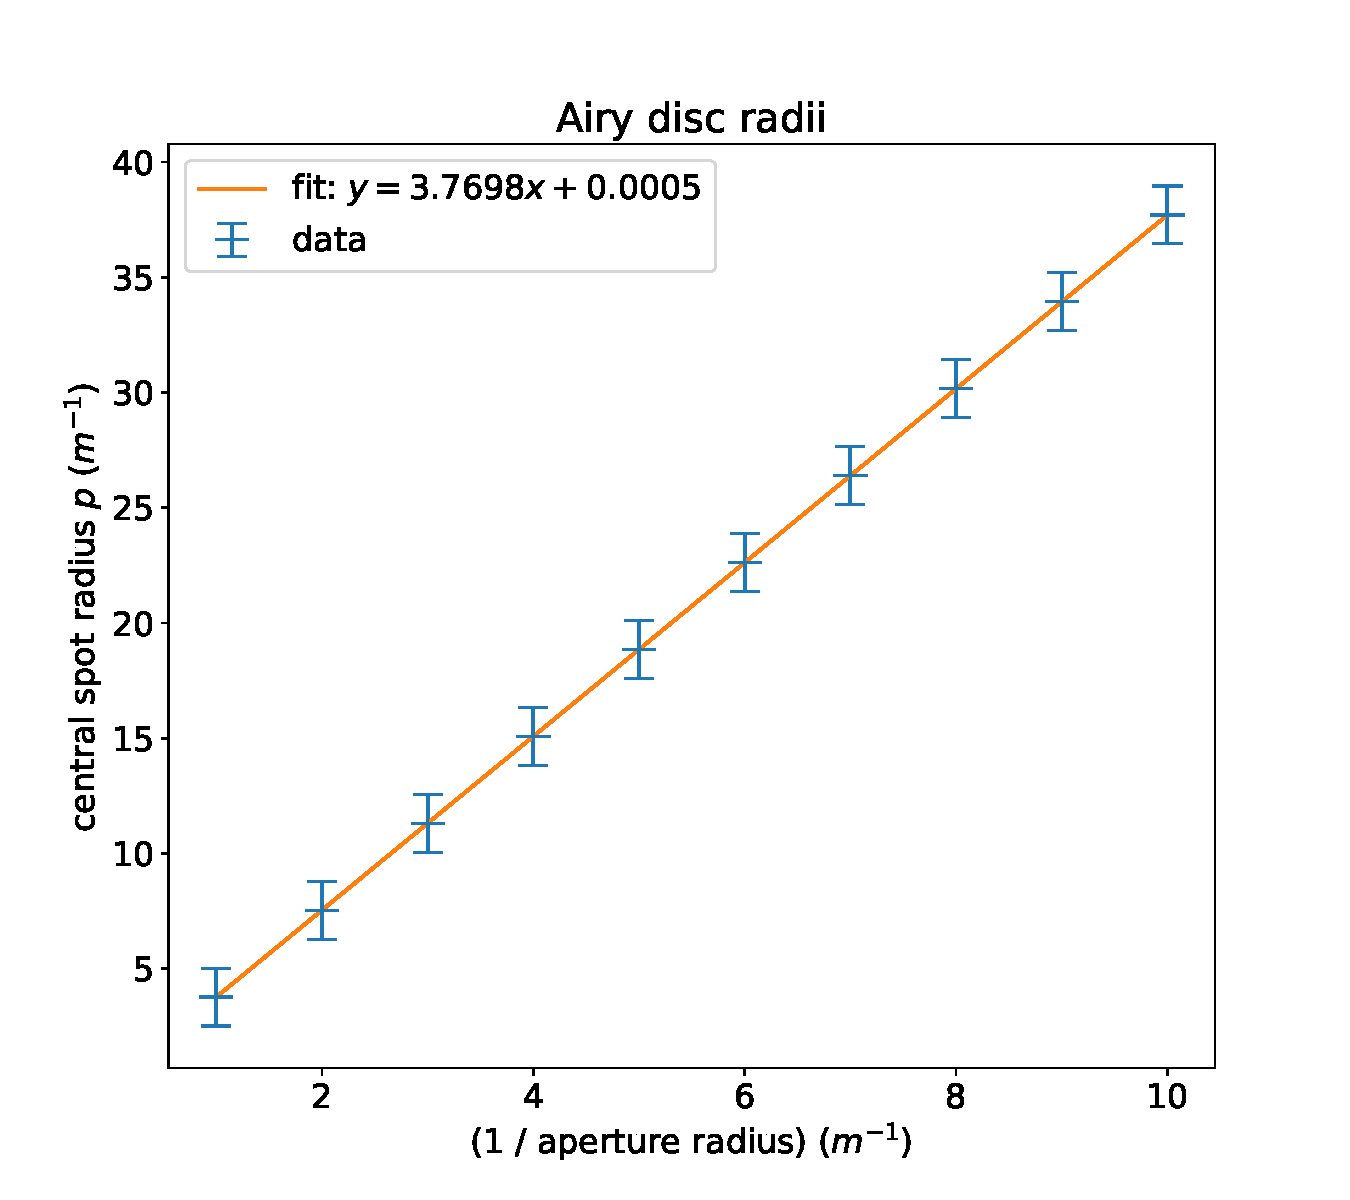
\includegraphics[width=\textwidth]{pictures/tests/airy.pdf}
        \caption{}\label{fig:test1:round}
    \end{subfigure}%
    \begin{subfigure}{0.5\textwidth}
        \centering
        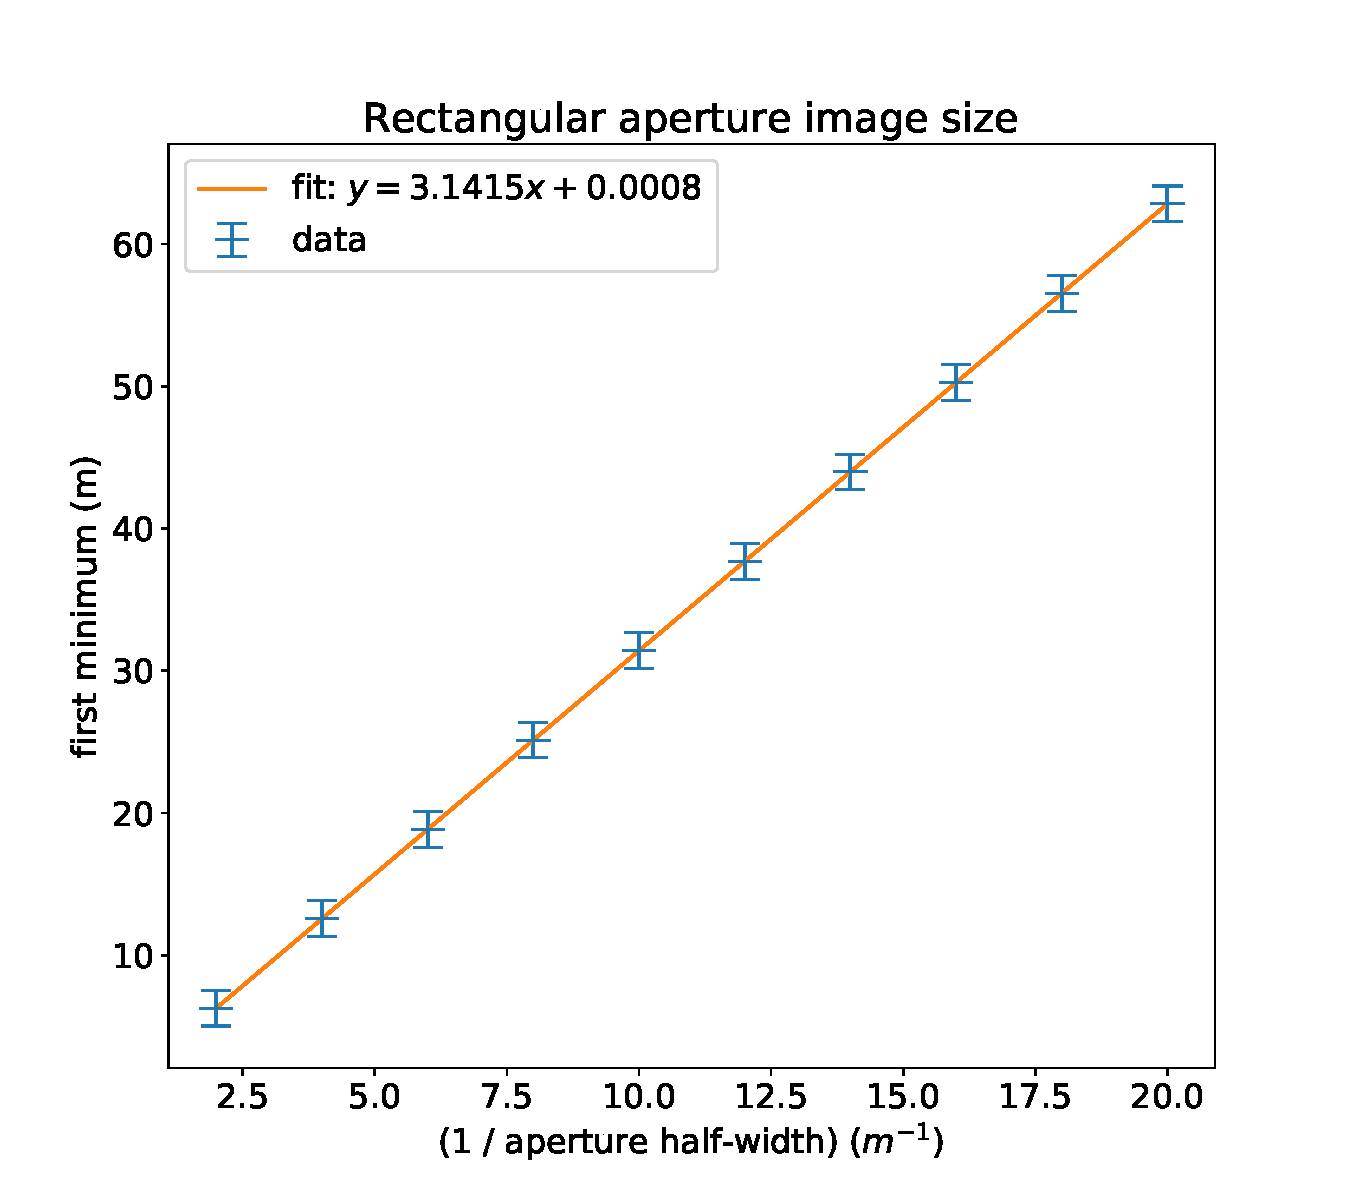
\includegraphics[width=\textwidth]{pictures/tests/rect.pdf}
        \caption{}\label{fig:test1:rect}
    \end{subfigure}
    \caption{Sizes of central spots as function of aperture size, for both round and rectangular apertures.}\label{fig:test1}
\end{figure}

\begin{figure}
    \centering
    \begin{subfigure}{0.5\textwidth}
        \centering
        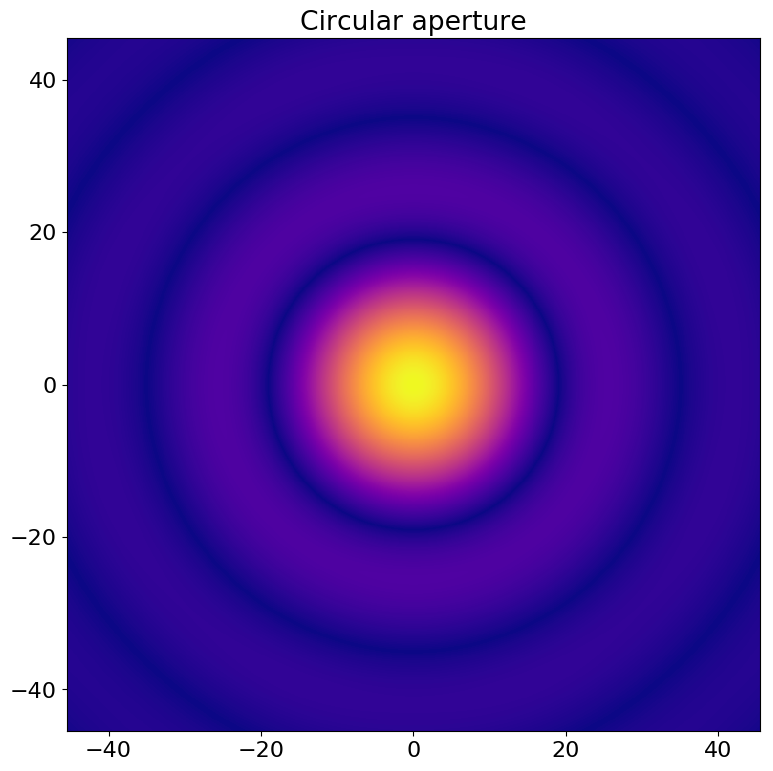
\includegraphics[width=\textwidth]{pictures/def/out0}
        \caption{}\label{fig:typ:round}
    \end{subfigure}%
    \begin{subfigure}{0.5\textwidth}
        \centering
        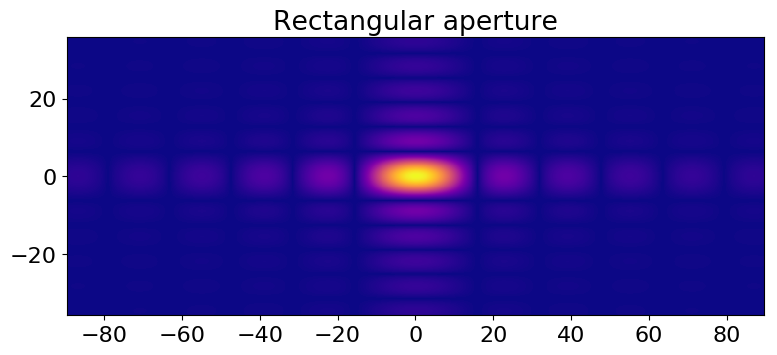
\includegraphics[width=\textwidth]{pictures/def/out1}
        \caption{}\label{fig:typ:rect}
    \end{subfigure}
    \caption{Typical diffraction patterns of circular and vertical rectangular apertures.}\label{fig:typ}
\end{figure}

First, I ran the program on series of circular and rectangular apertures described in \texttt{config/circular\_mins.txt} and \texttt{config/rectangle\_mins.txt}, expecting to see a linear relationship between the extent of the central maximum and the inverse of the aperture size (see Section~\ref{sec:analysis:test}). As seen in Figure~\ref{fig:test1}, these linear relationships hold. The line slopes are close to the expected values of $1.22\pi$ for the Airy disc and $\pi$ for rectangular shapes.

Figure~\ref{fig:typ} shows that the diffraction patterns look as expected. Most notably, the image from a vertical rectangle is longer along the horizontal axis, as expected from Equation~\ref{eqn:test_rect}.

\subsection{Gaussian Illumination}\label{sec:res:gauss}
\begin{figure}
    \centering
    \begin{subfigure}{0.49\textwidth}
        \centering
        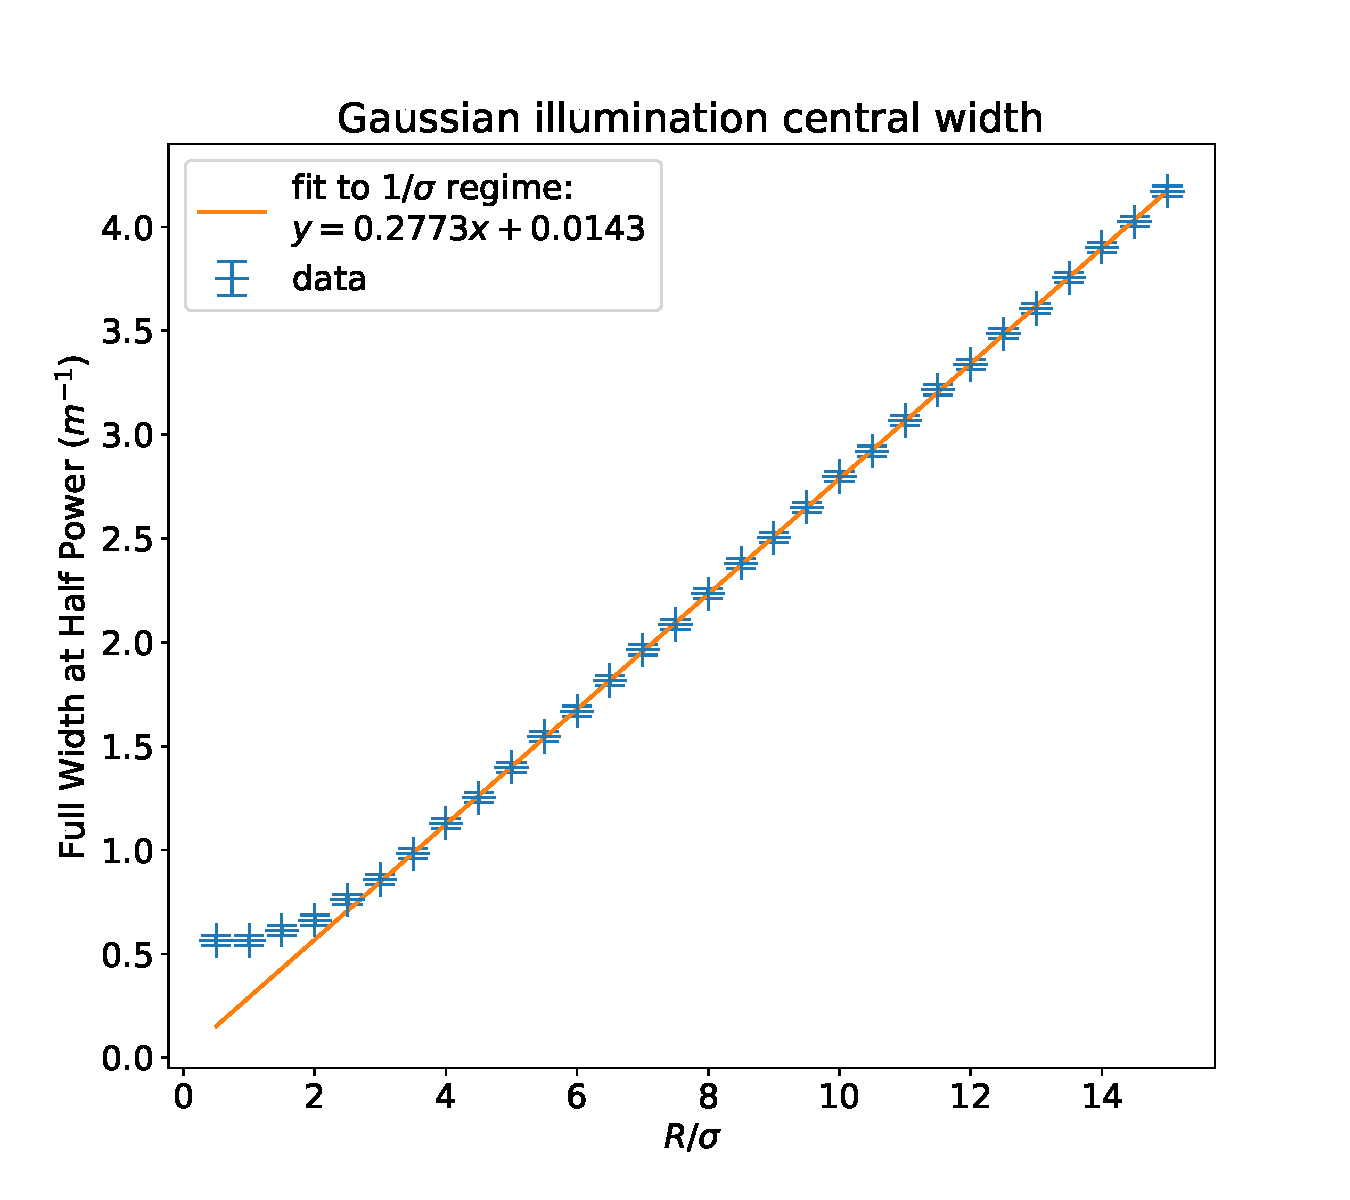
\includegraphics[width=\textwidth]{pictures/gauss/size.pdf}
        \caption{Dependence of full width at half maximum on aperture taper. The fit is for $R/\sigma > 3$.}\label{fig:gauss:size}
    \end{subfigure}%
    \hfill
    \begin{subfigure}{0.49\textwidth}
        \centering
        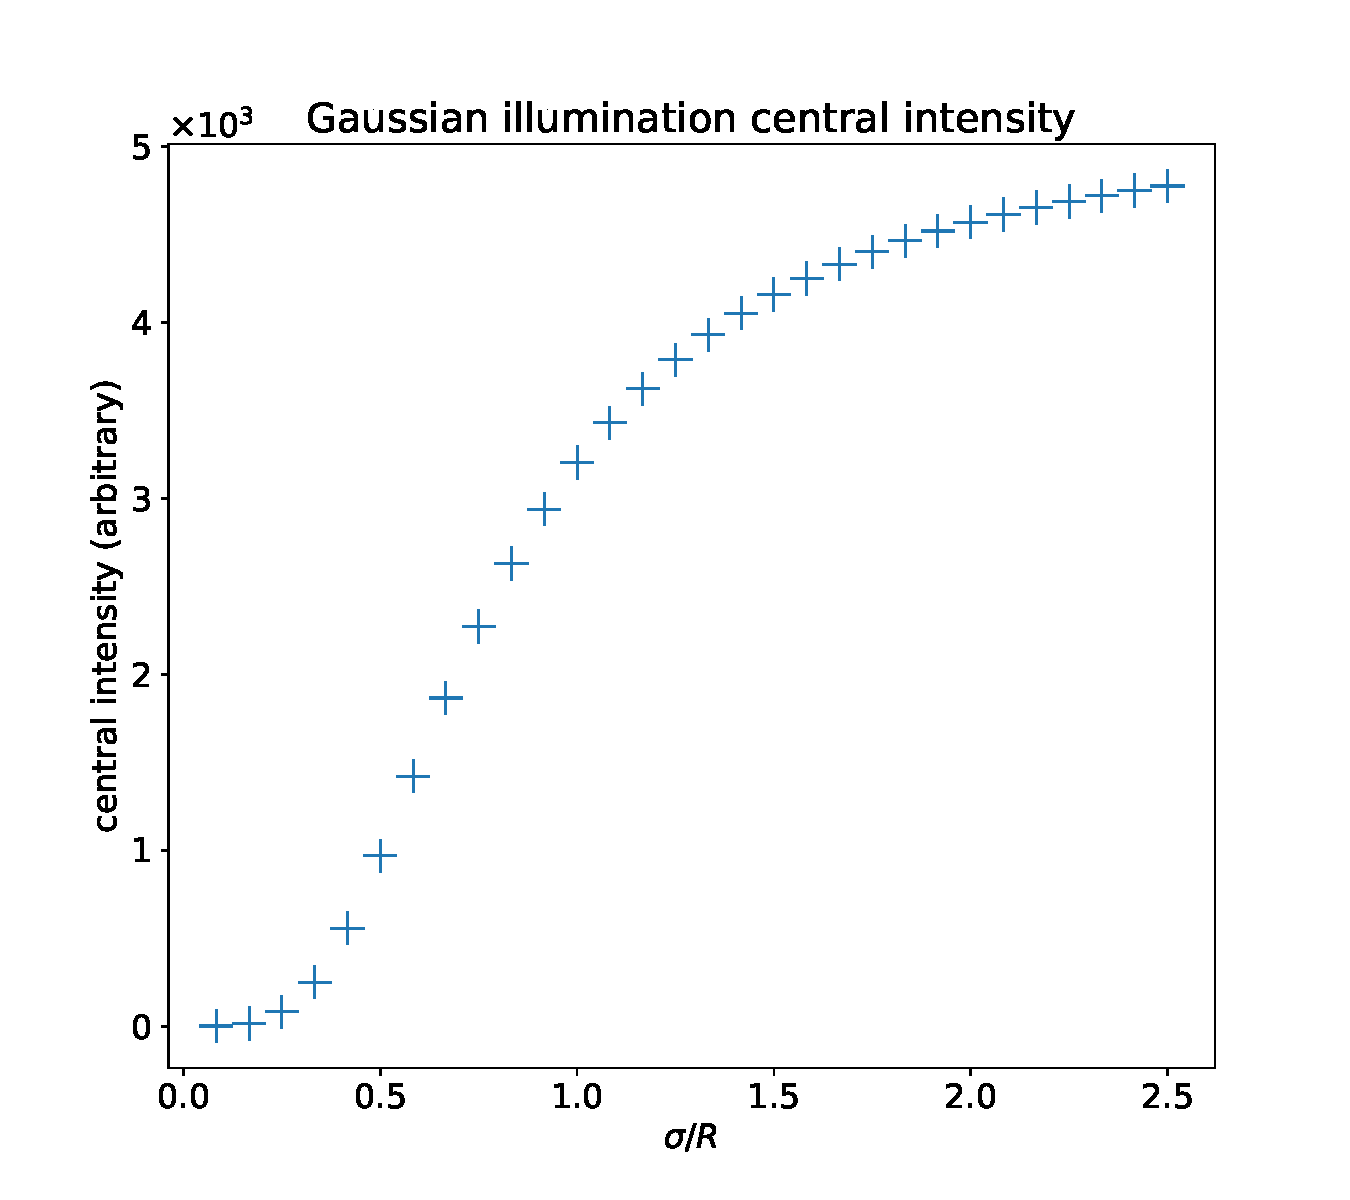
\includegraphics[width=\textwidth]{pictures/gauss/int.pdf}
        \caption{Central intensity variation with aperture taper.}\label{fig:gauss:int}
    \end{subfigure}
    \caption{Properties of Gaussian illumination diffraction pattern.}\label{fig:gauss}
\end{figure}

\begin{figure}
    \centering
    \begin{subfigure}{0.5\textwidth}
        \centering
        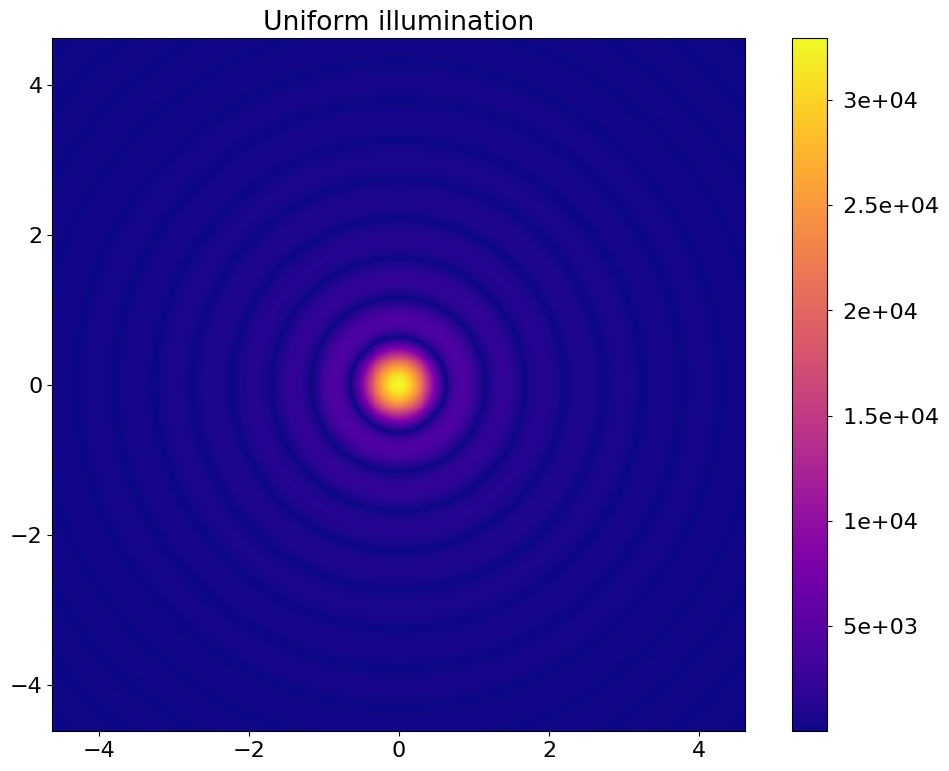
\includegraphics[width=\textwidth]{pictures/gauss/uniform.png}
        \caption{}\label{fig:gpic:uniform}
    \end{subfigure}%
    \begin{subfigure}{0.5\textwidth}
        \centering
        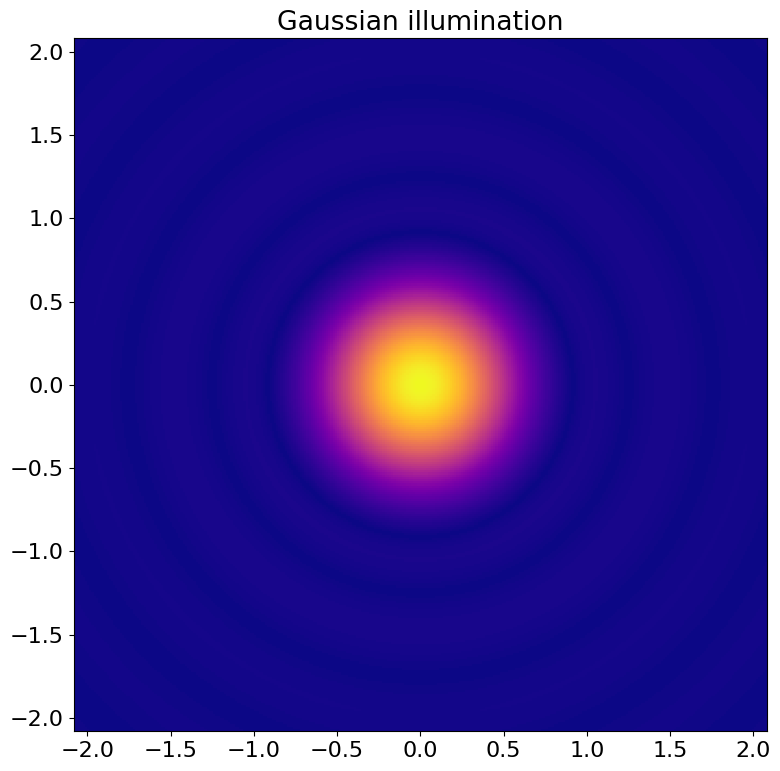
\includegraphics[width=\textwidth]{pictures/gauss/gaussian.png}
        \caption{}\label{fig:gpic:gauss}
    \end{subfigure}
    \caption{Amplitude diffraction patterns of two different illumination patterns of the same mirror of radius $R=\SI{6}{m}$. Note the different scales of the images.}\label{fig:gpic}
\end{figure}

Figure~\ref{fig:gauss} shows the results anticipated in Section~\ref{sec:analysis:taper}, especially the low and high $\sigma$ limits. At low $\sigma$, the $\R{FWHM} \propto 1/\sigma$, and the central intensity tends to zero. At high $\sigma$, both properties approach their uniform illumination values:
\begin{align*}
    \R{FWHP} &\rightarrow \SI{0.641 \pm 0.014}{\per\metre} \\
    I(0, 0) &\rightarrow \sim \num{30e3}.
\end{align*}

These results support the expected behaviour of Gaussian-illuminated apertures. Note that the shape in Figure~\ref{fig:gauss:int} is inherently hard to quantify since it results from the integral of a Gaussian, which has no analytical form.

Figure~\ref{fig:gpic} shows the images produced by illuminating the same mirror uniformly or with a taper. The uniformly lit mirror produces much sharper secondary rings. This suggests that the reason for using a taper is to concentrate more of the power in the central spot, and avoid the effects of the secondary peaks on image quality.

\subsection{Central hole}\label{sec:res:hole}
\begin{figure}
    \centering
    \begin{minipage}{0.48\textwidth}
        \centering
        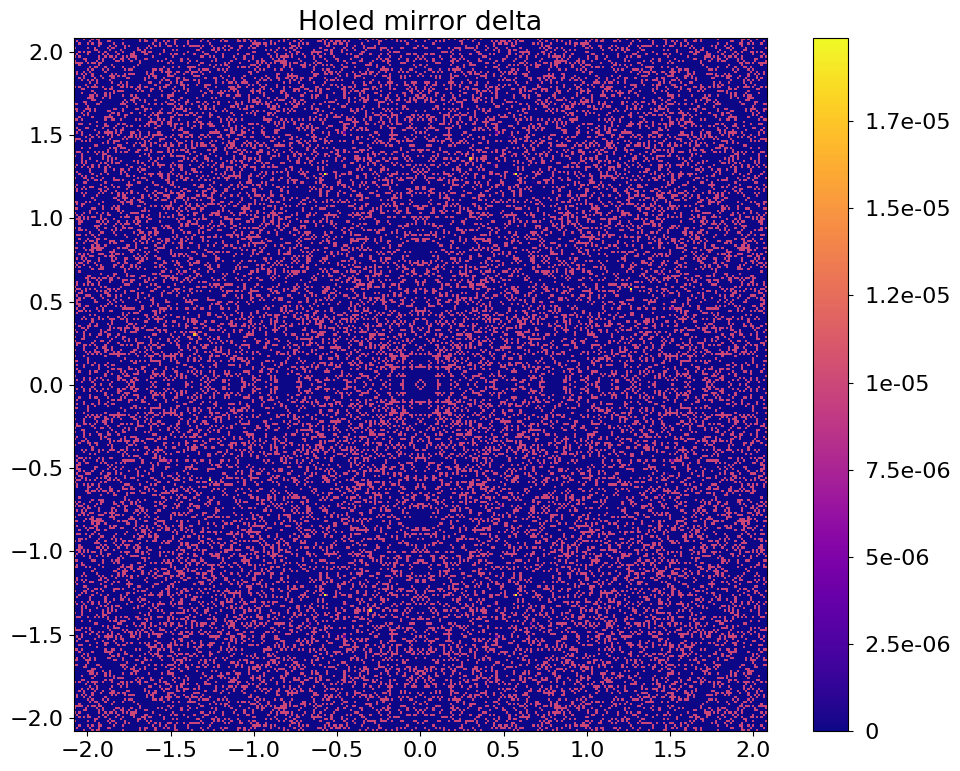
\includegraphics[width=\textwidth]{pictures/hole/delta2.png}
        \caption{The diffraction pattern of a mirror with a central hole of radius $r=\SI{0.5}{m}$ was subtracted from the difference of diffraction patterns of a complete mirror and just the central hole.}\label{fig:hole-delta}
    \end{minipage}%
    \hfill
    \begin{minipage}{0.48\textwidth}
        \centering
        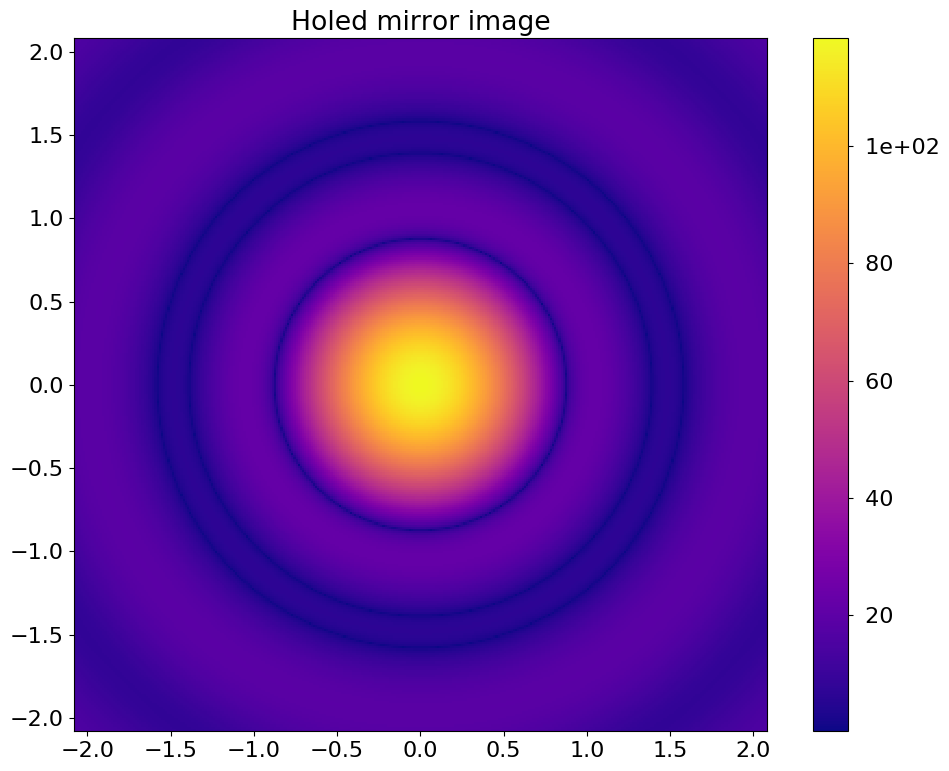
\includegraphics[width=\textwidth]{pictures/hole/image.png}
        \caption{diffraction pattern of holed mirror. The amplitude was raised to the power $1/2$ for better visibility.}\label{fig:hole}
    \end{minipage}
\end{figure}

The diffraction pattern of a mirror with a central hole is seen in Figure~\ref{fig:hole}. The expected irregular rings are visible.

Figure~\ref{fig:hole-delta} shows the results of the calculation suggested in Section~\ref{sec:analysis:hole}. We can see the amplitude of the difference reaching at most around \num{2e-5}. In the original diffraction patterns, the central amplitude is on the order of $10^4$, so indeed the two patterns are equal to a very high accuracy. The differences are on the order of the precision to which the numbers were printed before plotting, around $10^{-6}$.

This confirms that the F.T. operations we use are linear to a good accuracy.

\subsection{Random errors}\label{sec:res:rand}
\begin{figure}
    \centering
    \begin{subfigure}{0.45\textwidth}
        \centering
        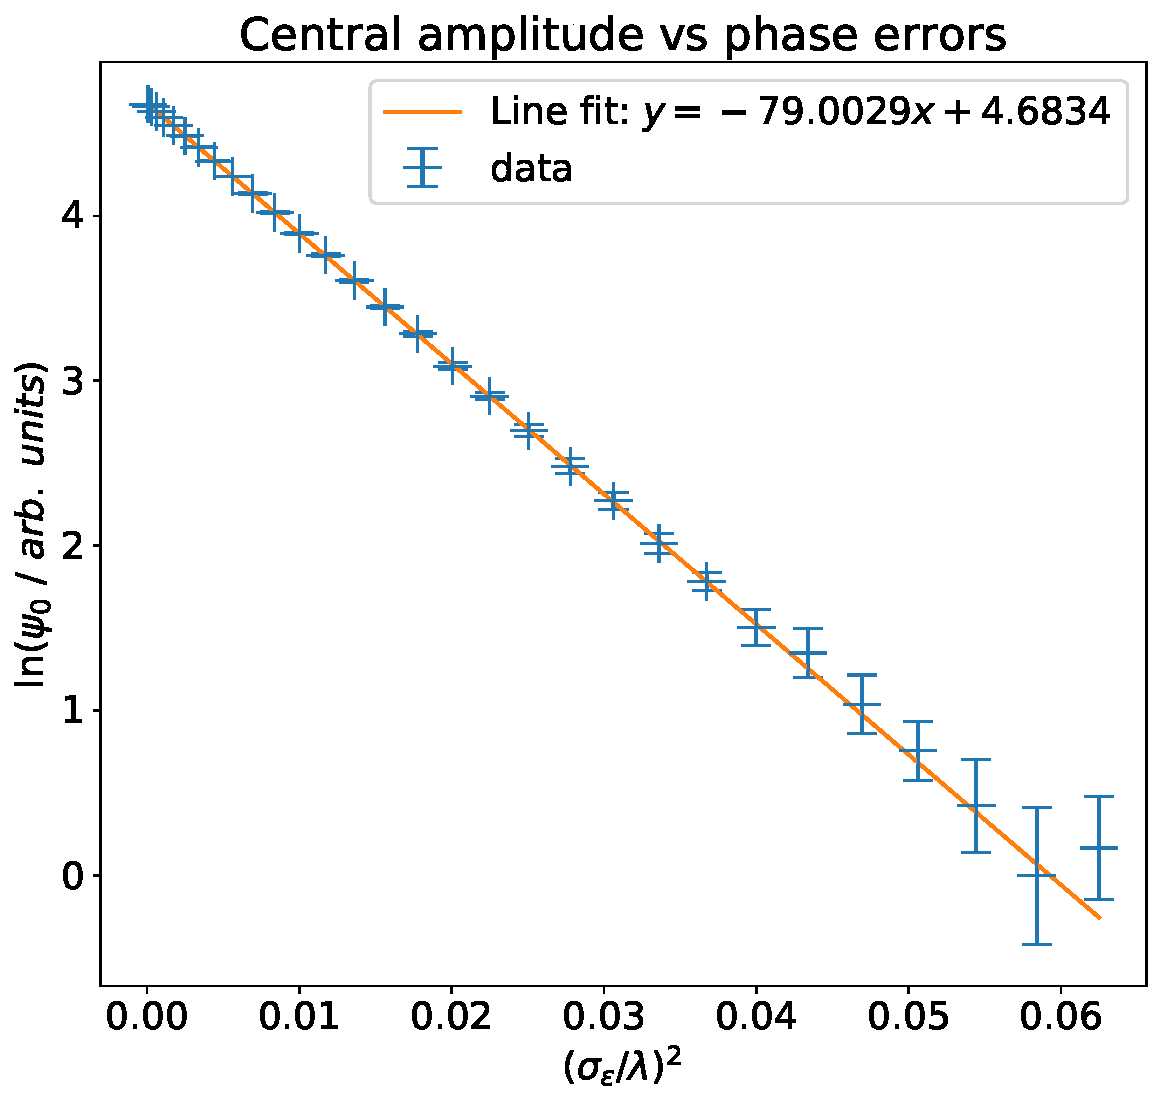
\includegraphics[width=\textwidth]{pictures/rand/int}
        \caption{dependence of the central amplitude on phase (wavefront) error. Note logarithmic scale of the vertical axis.}\label{fig:rand:int}
    \end{subfigure}%
    \hfill
    \begin{subfigure}{0.45\textwidth}
        \centering
        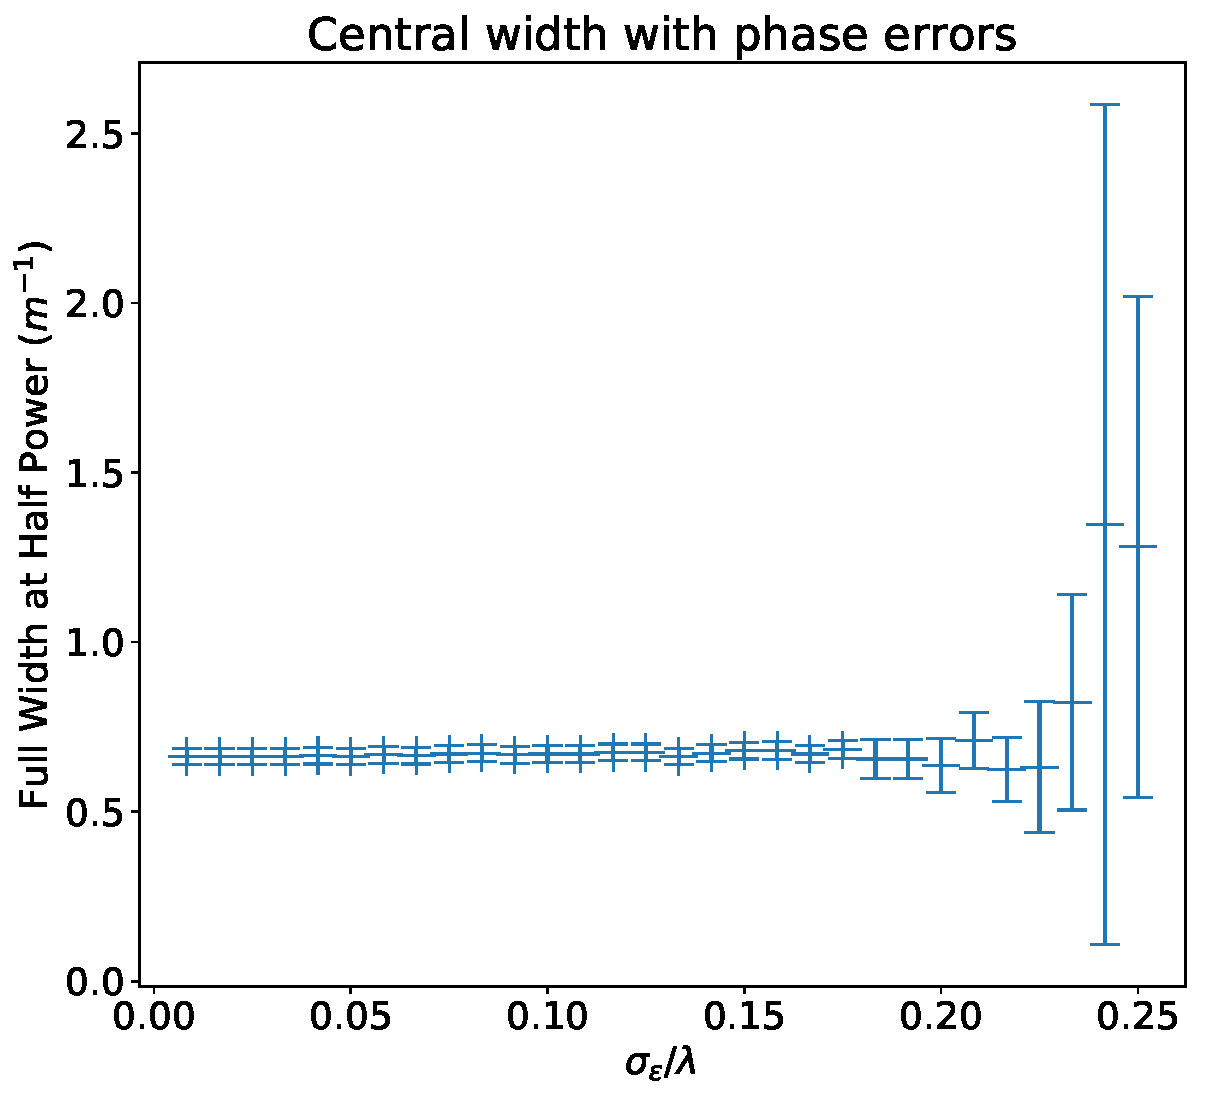
\includegraphics[width=\textwidth]{pictures/rand/size}
        \caption{(lack of) relationship of full-width-at-half-power with random phase errors.}\label{fig:rand:size}
    \end{subfigure}
    \caption{}\label{fig:rand}
\end{figure}

Typical mirror and image shapes for random phase errors are seen in Figure~\ref{fig:randpic}.

Figure~\ref{fig:rand} shows how properties of the image are affected by random errors. The width of the central disc is unaffected, but the central amplitude ($\psi_0$) decreases with the RMS error $\sigma_\eps$. When $4\pi\sigma_\eps / \lambda = \sigma_\ph \rightarrow \pi$, the amplitude tends to zero. The linear relationship in Fig.~\ref{fig:rand:int} indicates that the amplitude is a Gaussian function of the wavefront error:
\begin{equation}\label{eqn:amp-v-rms}
    \psi_0 \propto \exp \left( - \frac{(\sigma_\eps / \lambda)^2}{2 \sigma_\psi^2} \right),
\end{equation}
with
\begin{equation}
    \sigma_\psi = \num{79.56 \pm 0.03 e-3}
\end{equation}
given by the line slope.

The implication for telescopes is that larger wavefront errors will decrease the apparent brightness of the observed objects.

\subsection{Error correlation tests}\label{sec:res:rms}
\begin{figure}
    \centering
    \begin{subfigure}{0.5\textwidth}
        \centering
        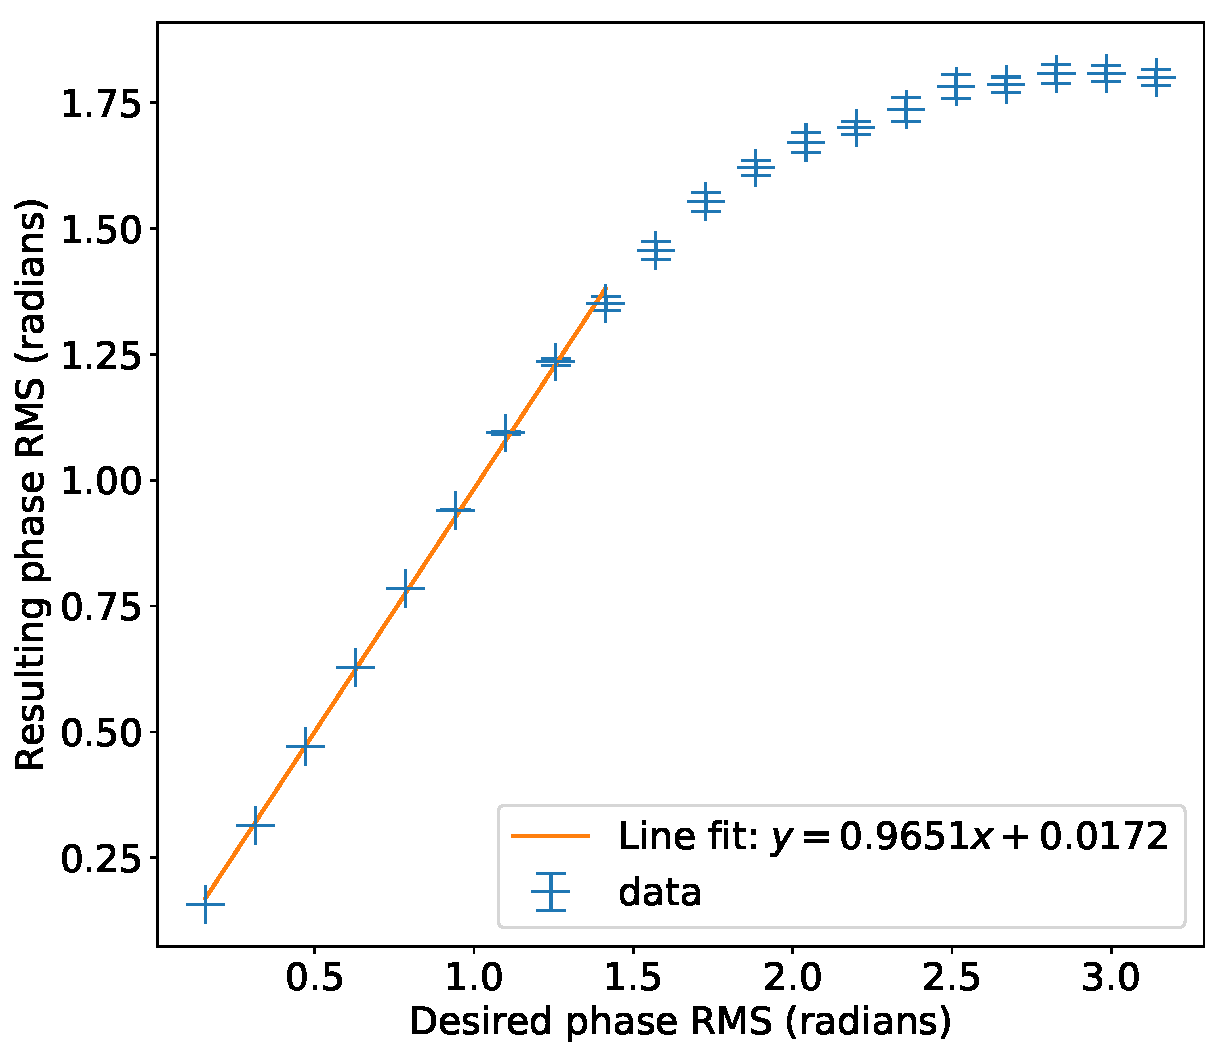
\includegraphics[width=0.95\textwidth]{pictures/rmstest/depth}
        \caption{}\label{fig:rms:depth}
    \end{subfigure}%
    \begin{subfigure}{0.5\textwidth}
        \centering
        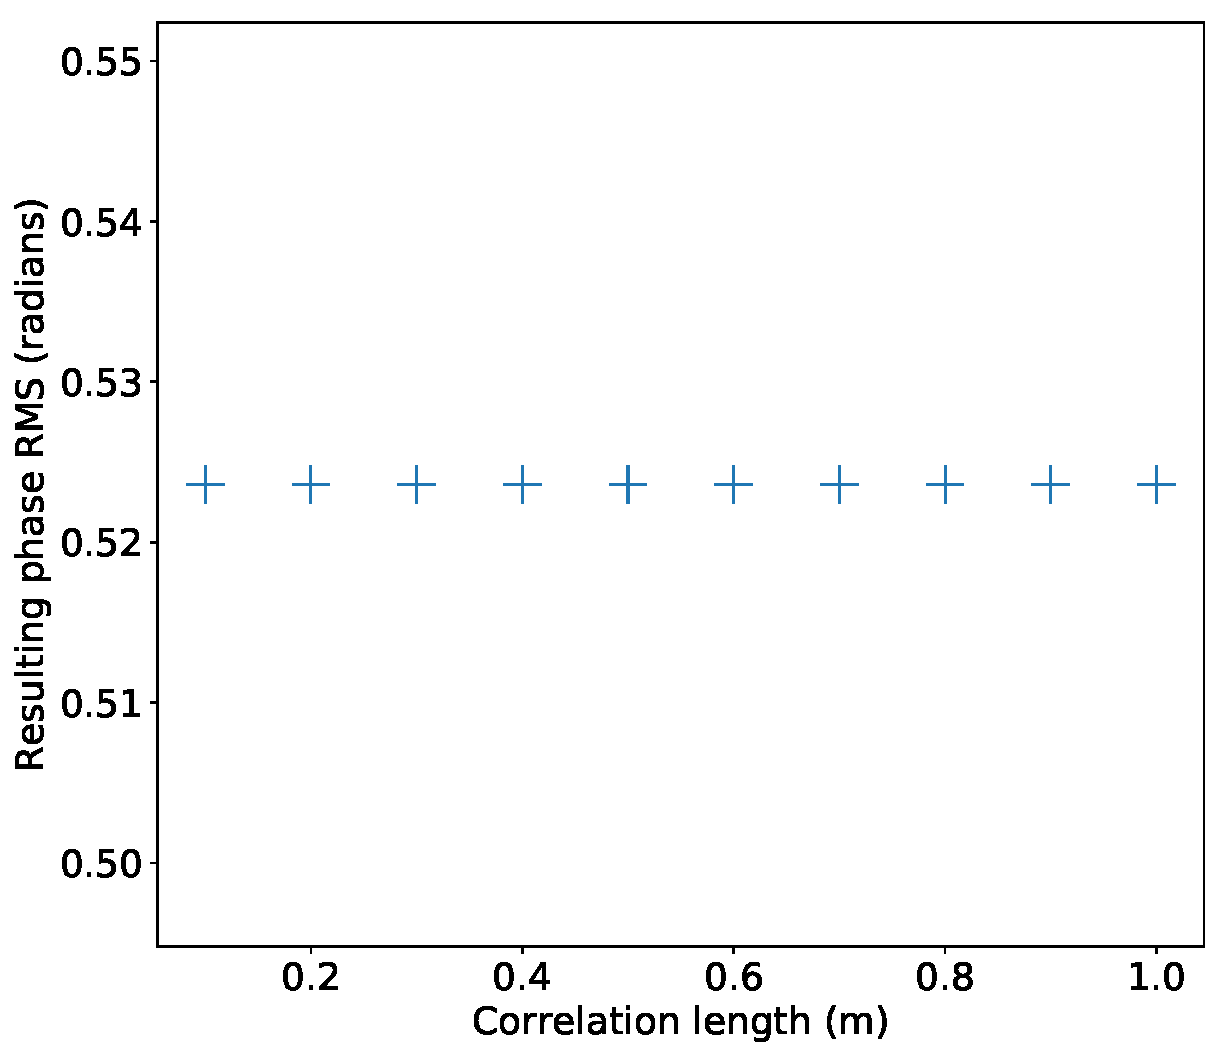
\includegraphics[width=0.95\textwidth]{pictures/rmstest/l_corr}
        \caption{}\label{fig:rms:length}
    \end{subfigure}
    \caption{dependence of RMS (root mean square) phase on desired RMS and correlation length.}\label{fig:rms}
\end{figure}

In Figure~\ref{fig:rms:depth} we see that the produced RMS phase error is close to the desired one for phases of up to $\frac{\pi}{2}$. It saturates to about \SI{1.8}{\radian} at larger desired $\sigma_\eps$, probably due to some numbers falling outside the $(-\pi,\ \pi)$ range, and overflowing when they are converted to complex phase. This is expected behaviour.

Figure~\ref{fig:rms:length} shows that the RMS wavefront error does not depend on correlation length, which confirms normalisation is correct.

\subsection{Spatially correlated errors}\label{sec:res:corr}
\begin{figure}
    \centering
    \begin{minipage}{0.48\textwidth}
        \centering
        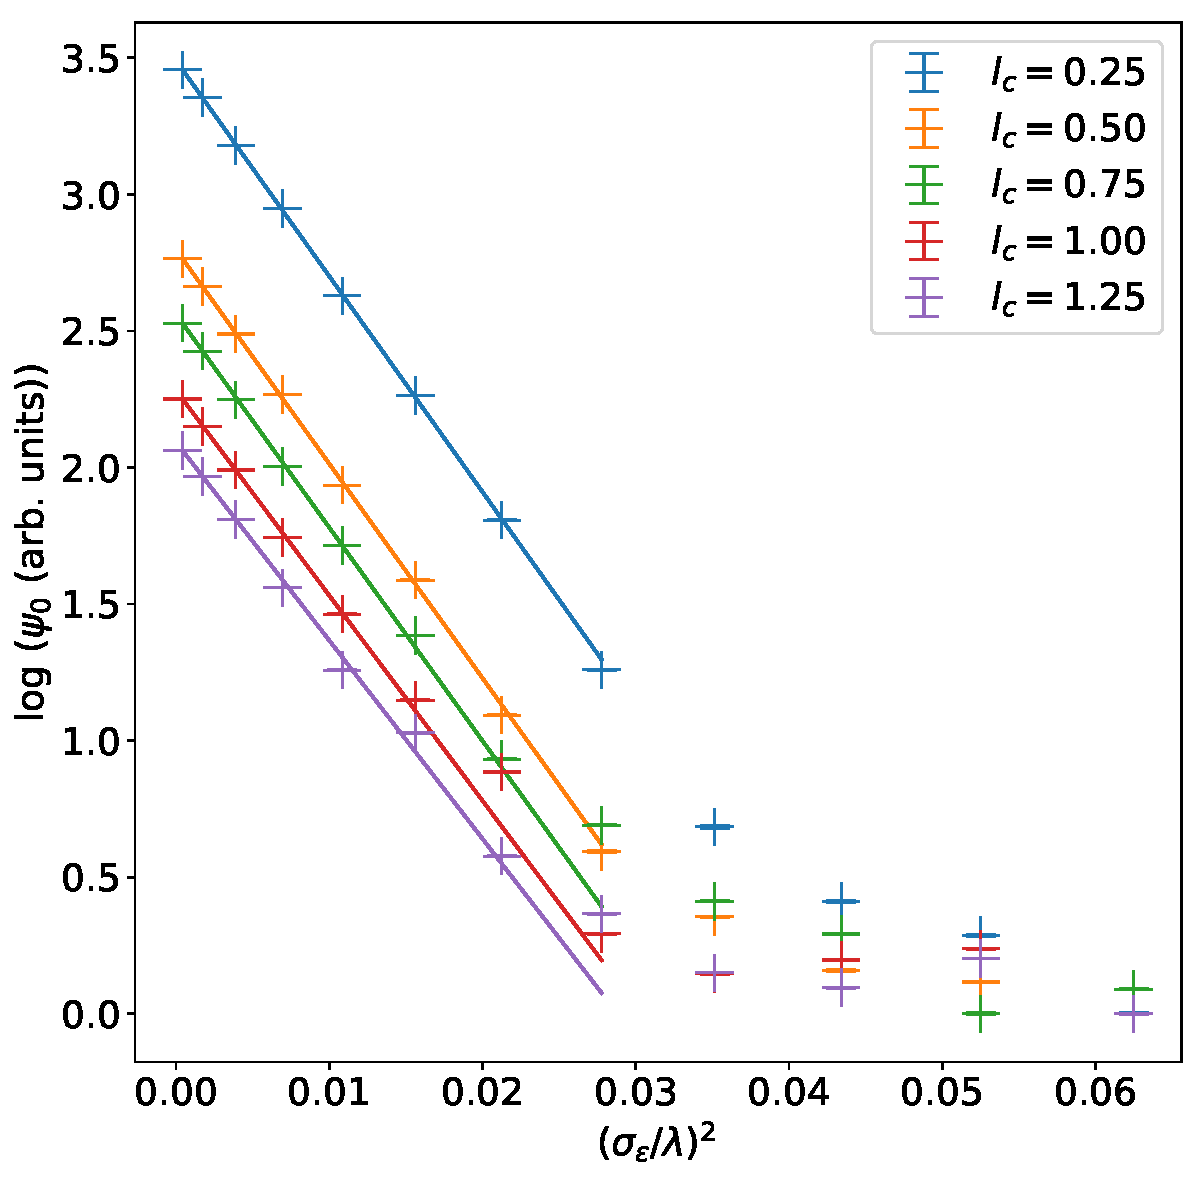
\includegraphics[width=\textwidth]{pictures/corr/amp.pdf}
        \caption{dependence of central amplitude on the RMS of correlated phase errors, for different defect lengths (in meters). Values are normalised to the smallest in the series.}\label{fig:corr:amps}
    \end{minipage}\hfill
    \begin{minipage}{0.48\textwidth}
        \centering
        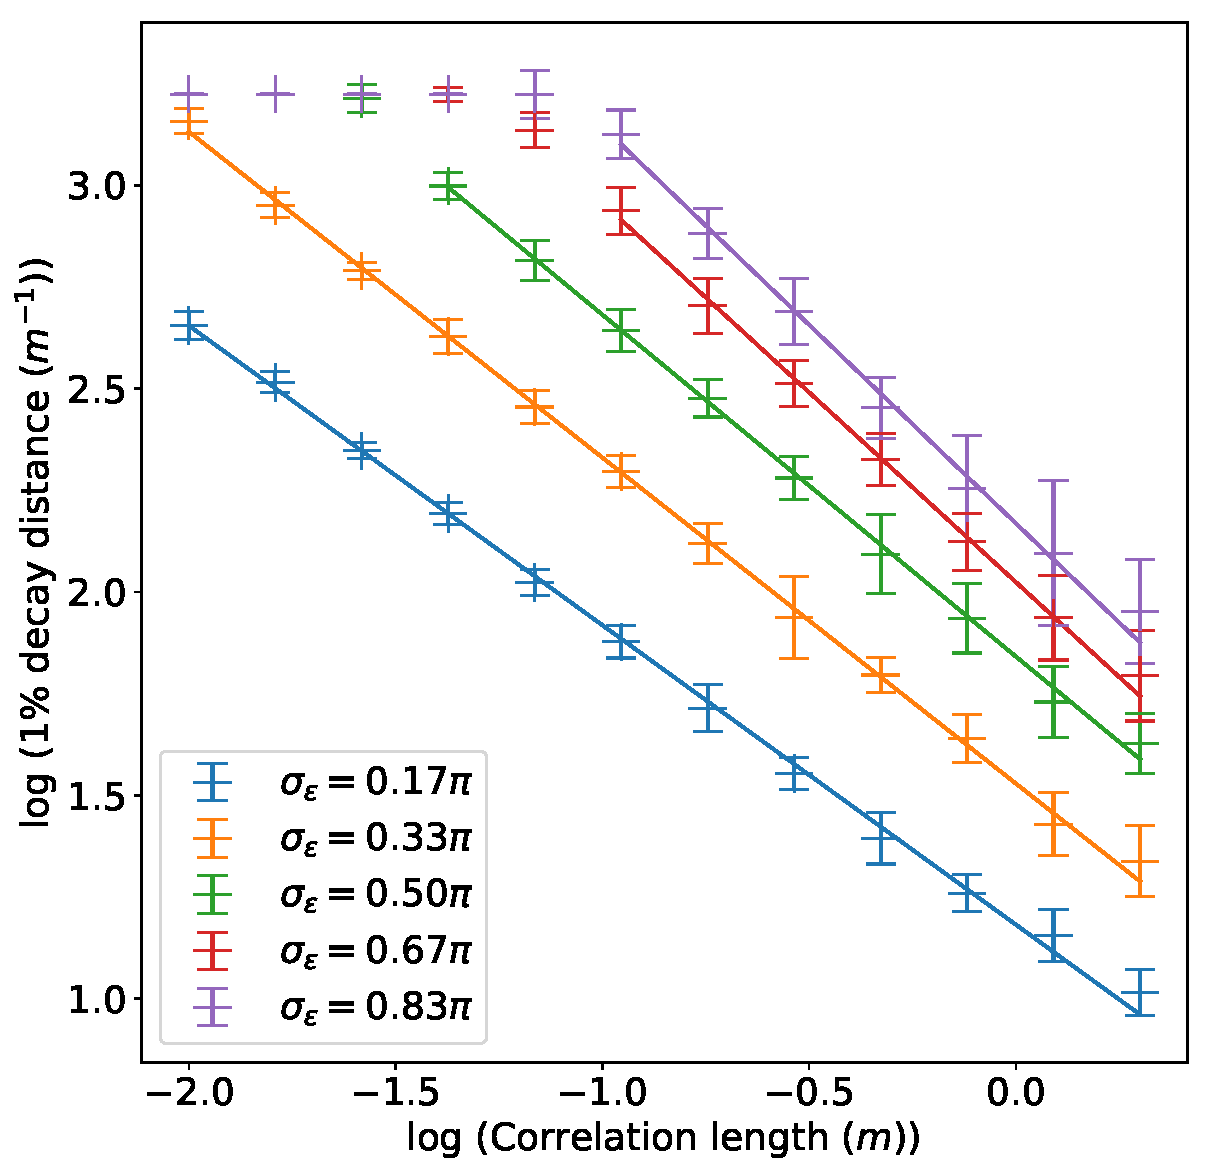
\includegraphics[width=\textwidth]{pictures/corr/dist.pdf}
        \caption{farthest distance from the centre where an amplitude at least \SI{1}{\percent} of the central one is found, as a function of error correlation length (or defect `width'). Error bars are the standard deviation of 20 runs. Three of the series are seen to saturate at the same value, reaching the maximum extent of the discrete Fourier transform.}\label{fig:corr:dist}
    \end{minipage}
\end{figure}

\begin{figure}
    \centering
    \begin{minipage}{0.48\textwidth}
        \centering
        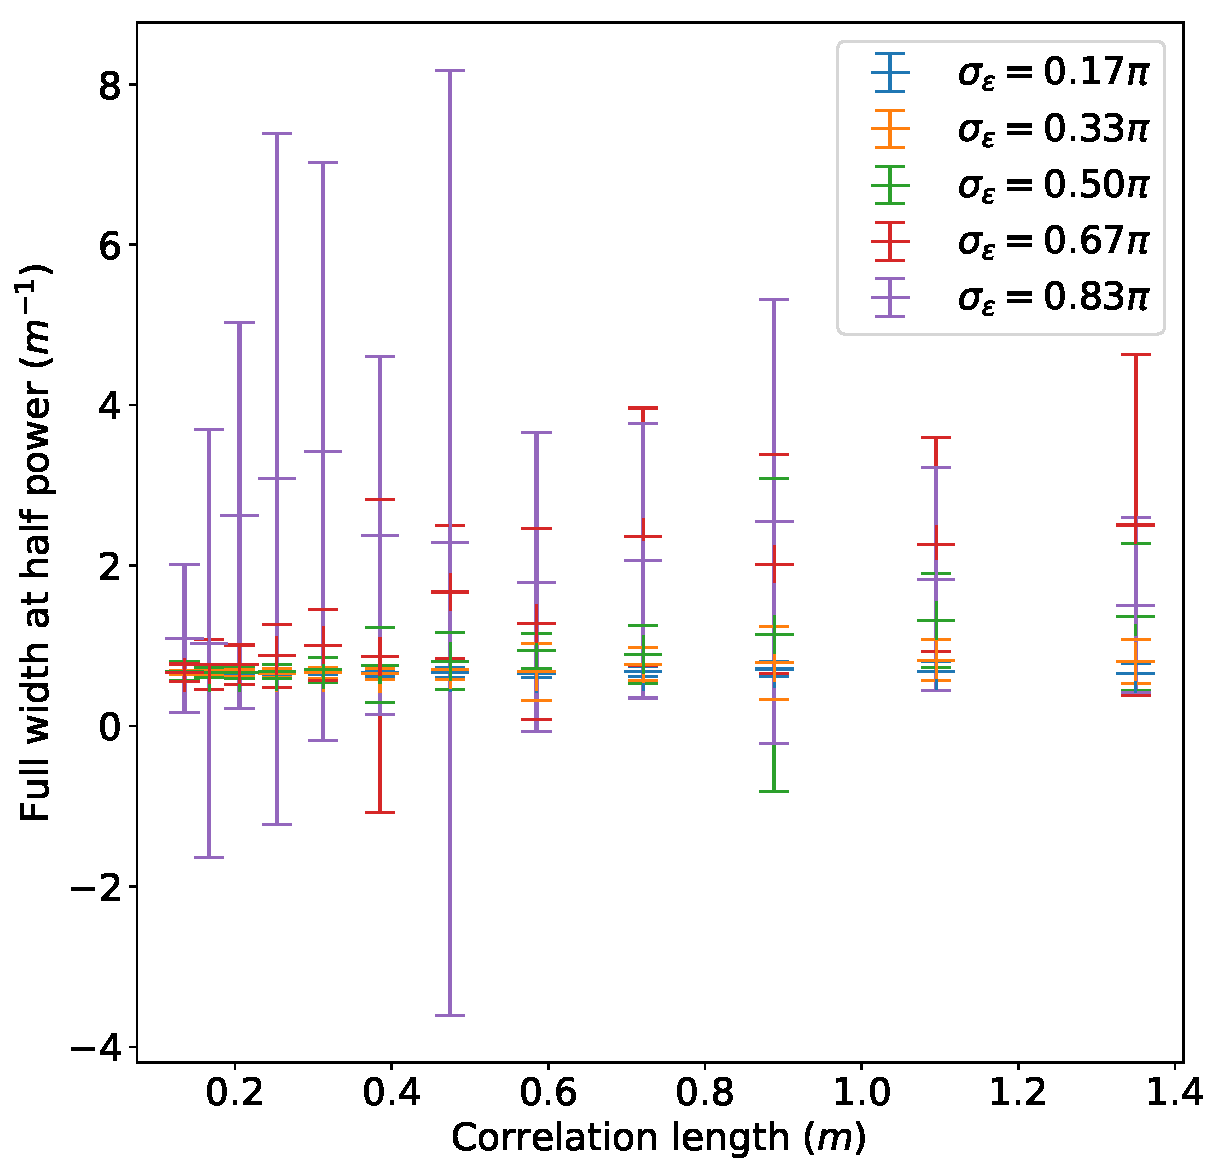
\includegraphics[width=\textwidth]{pictures/corr/fwhp.pdf}
    \end{minipage}\hfill
    \begin{minipage}{0.48\textwidth}
        \caption{the full width at half power as a function of correlation length, for different values of the RMS wavefront error. Error bars are the standard deviation of 20 runs.}\label{fig:corr:fwhp}
    \end{minipage}
\end{figure}

\begin{table}[!h]
    \centering
    \begin{tabular}{ c | c }
        Defect length $l_c$ & Decay width $\sigma_\psi$ \\
        \hline
        \SI{0.25}{m} & $\num{79.6 \pm 0.2 e-3}$ \\
        \SI{0.50}{m} & $\num{79.8 \pm 0.3 e-3}$ \\
        \SI{0.75}{m} & $\num{80.0 \pm 0.8 e-3}$ \\
        \SI{1.00}{m} & $\num{81.6 \pm 0.9 e-3}$ \\
        \SI{1.25}{m} & $\num{83 \pm 1 e-3}$ \\
    \end{tabular}
    \caption{decay widths of on-axis amplitude with wavefront error.}\label{tab:corr-amp}
\end{table}

\begin{table}[!h]
    \centering
    \begin{tabular}{ c | c }
        RMS phase ($4\pi\sigma_\eps/\lambda$) & exponent ($n$) \\
        \hline
        $\SI{\pi/6}{\radian}$ & $\num{0.736 \pm 0.008}$ \\
        $\SI{\pi/3}{\radian}$ & $\num{0.801 \pm 0.008}$ \\
        $\SI{\pi/2}{\radian}$ & $\num{0.84 \pm 0.01}$ \\
        $\SI{2\pi/3}{\radian}$ & $\num{0.93 \pm 0.02}$ \\
        $\SI{5\pi/6}{\radian}$ & $\num{0.98 \pm 0.04}$ \\
    \end{tabular}
    \caption{exponents in the relation of \SI{1}{\percent} decay distance with defect correlation length.}\label{tab:corr-dist}
\end{table}

Finally, we explore the effects of finite-width defects in the mirror surface. Figure~\ref{fig:corrpic} shows some typical diffraction patterns at different defect lengths.

Figure~\ref{fig:corr:amps} shows that the exponential relationship in Equation~\ref{eqn:amp-v-rms} does not hold for the entire range $4\pi\sigma_\eps/\lambda \in (0, \pi)$, but rather only to around $3\pi/4$. The decay rates $\sigma_\psi$ of amplitude with wavefront error are in Table~\ref{tab:corr-amp}. At small correlation lengths, these are similar to the one found in Section~\ref{sec:res:rand}, which is good limiting behaviour.

Another interesting relation emerges: I measured the maximum distance from the centre it takes the amplitude to decay to \SI{1}{\percent} of the maximum value. The results in Figure~\ref{fig:corr:dist} show that this decay distance ($p_{1/100}$) decreases with the defect width, and increases with the wavefront error, i.e.\ with the depth. The fitted lines show that:
\begin{equation}
    p_{1/100} \propto l_c^{-n}, \qq{with} n \in (2/3, 1).
\end{equation}
The calculated values of the exponent $n$ are in Table~\ref{tab:corr-dist}.

For telescope manufacturing, the implication is that, at the same wavefront precision, many narrow defects will spread energy farther from the centre of the diffraction pattern compared to fewer wider defects. In the light of the inverse relationship between the sizes of mirror shapes and their Fourier Transforms, this makes intuitive sense.

Interestingly, the full width at half-power of the central diffraction peak was found to be unaffected by the correlation length, at least in the range of lengths studied (see Figure~\ref{fig:corr:fwhp}). A possible explanation is that, since the typical size of the defects is smaller than the mirror size ($l_c \in$ \SIrange{0.1}{1.5}{\metre}, while $R = \SI{6}{\metre}$), their effects on the image are on a larger length scale than the central maximum.

The on-axis amplitude was also found to not vary with the defect size. If the normalisation in Figure~\ref{fig:corr:amps} is removed, all the data series approximately coincide. Again, the intuitive explanation would be that, since $\psi_0$ is the integral of the aperture function (i.e.\ in Equation~\ref{eqn:diff} the exponent is $0$), the spatial distribution of complex phase is not important.

\newgeometry{left=0.5cm, right=0.5cm}
\begin{figure}
    \centering
    \begin{subfigure}{0.5\textwidth}
        \begin{minipage}{0.5\textwidth}
            \centering
            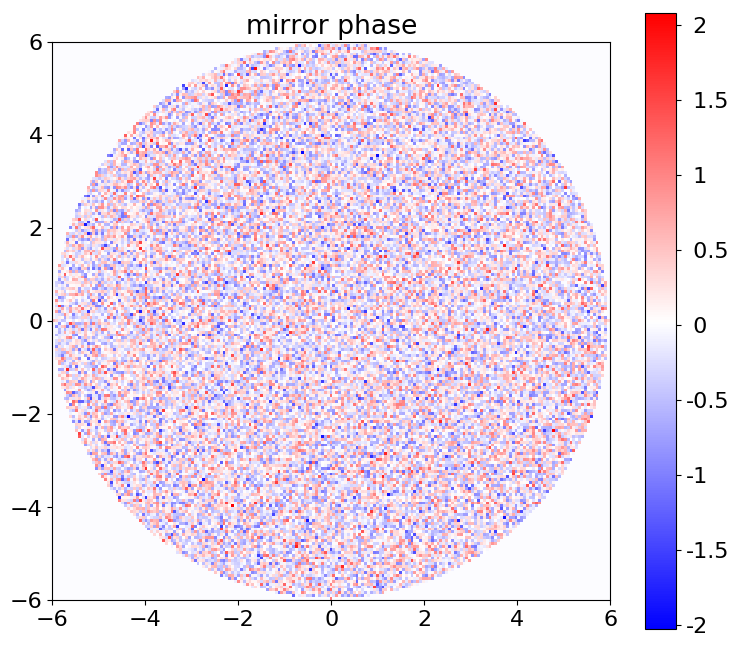
\includegraphics[width=\textwidth]{pictures/error_pics/errors0in_phase.png}
        \end{minipage}%
        \hfill
        \begin{minipage}{0.5\textwidth}
            \centering
            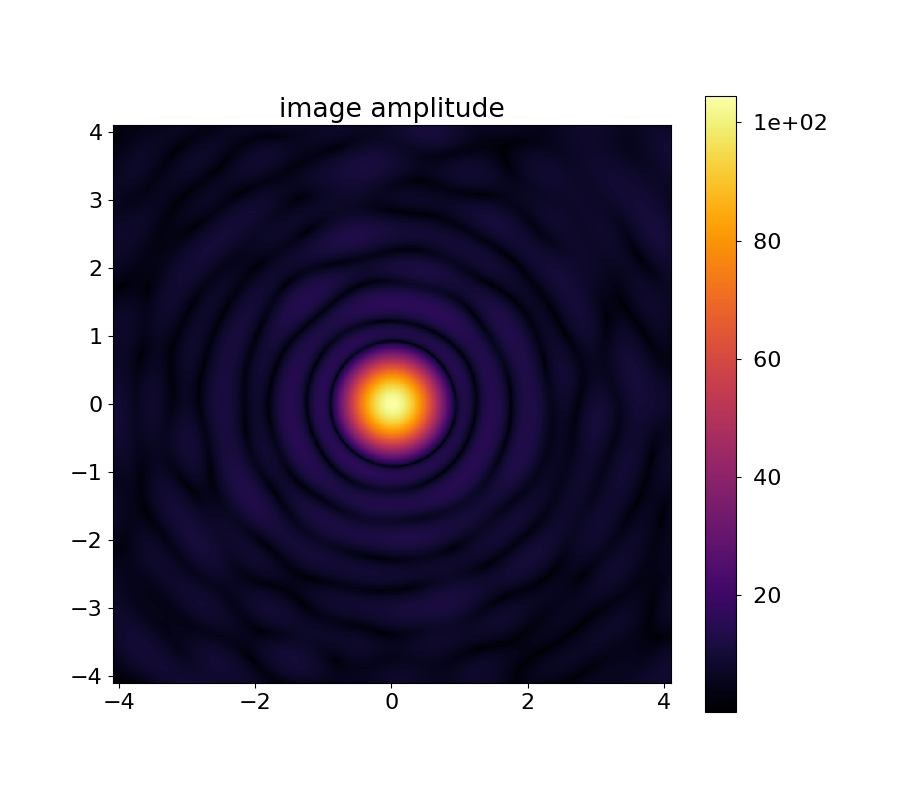
\includegraphics[width=\textwidth]{pictures/error_pics/errors0out_abs.png}
        \end{minipage}
        \caption{$\sigma_{\eps} = \pi/6$}\label{fig:randpic:1}
    \end{subfigure}%
    \hfill
    \begin{subfigure}{0.5\textwidth}
        \begin{minipage}{0.5\textwidth}
            \centering
            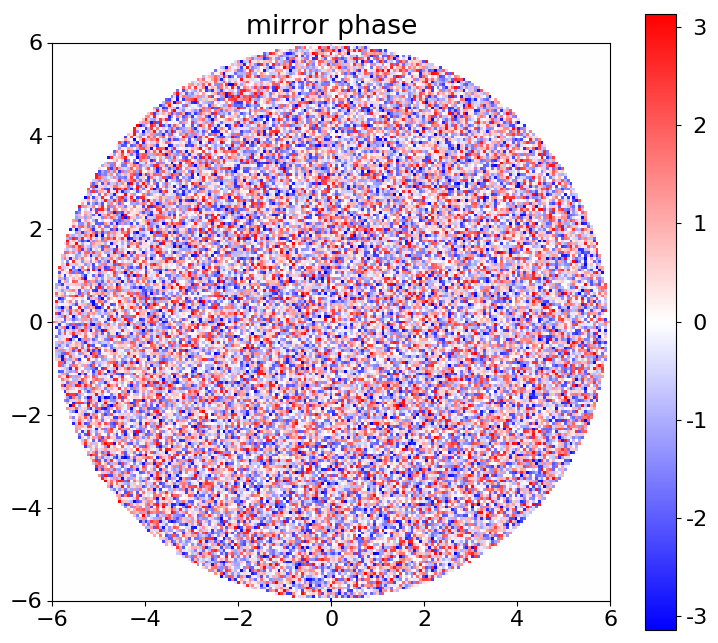
\includegraphics[width=\textwidth]{pictures/error_pics/errors1in_phase.png}
        \end{minipage}%
        \hfill
        \begin{minipage}{0.5\textwidth}
            \centering
            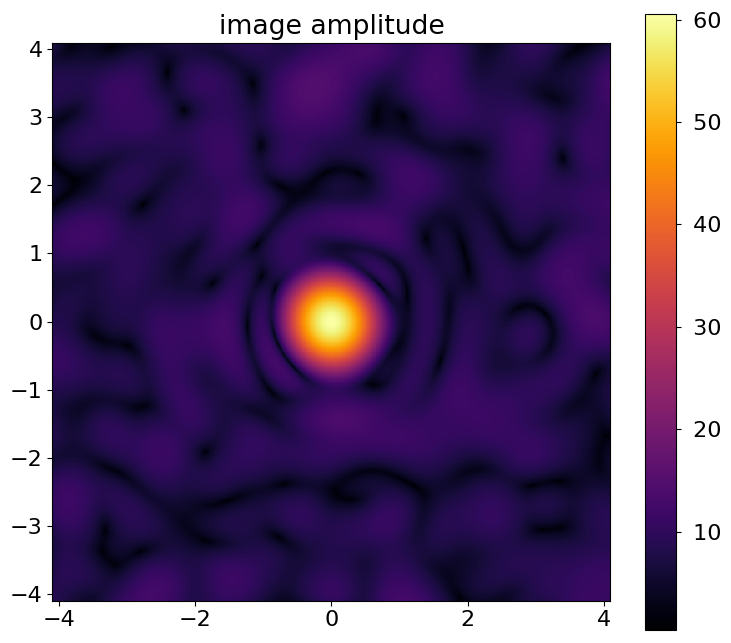
\includegraphics[width=\textwidth]{pictures/error_pics/errors1out_abs.png}
        \end{minipage}
        \caption{$\sigma_{\eps} = \pi/2$}\label{fig:randpic:2}
    \end{subfigure}
    \caption{Typical random error aperture functions and resulting diffraction patterns. Amplitudes are raised to the power $1/2$ to make features easier to see.}\label{fig:randpic}
\end{figure}

\begin{figure}
    \centering
    \begin{subfigure}{0.5\textwidth}
        \begin{minipage}{0.5\textwidth}
            \centering
            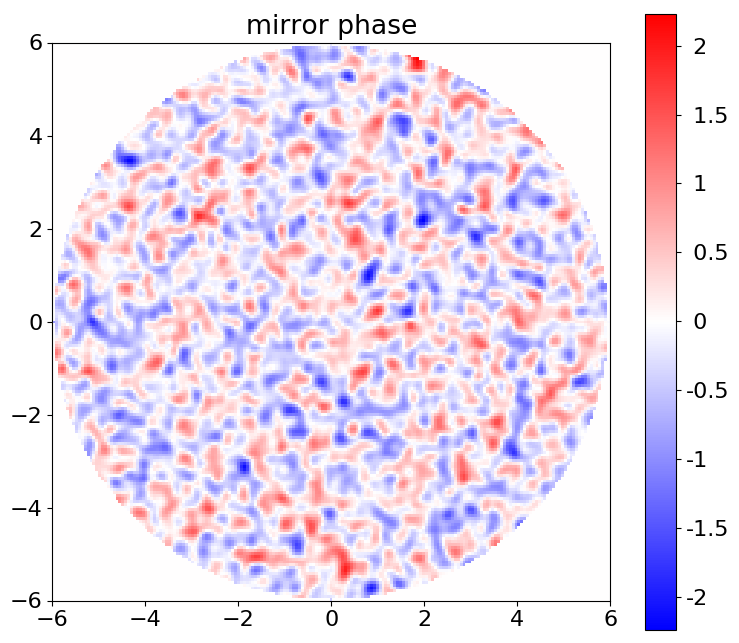
\includegraphics[width=\textwidth]{pictures/error_pics/errors2in_phase.png}
        \end{minipage}%
        \begin{minipage}{0.5\textwidth}
            \centering
            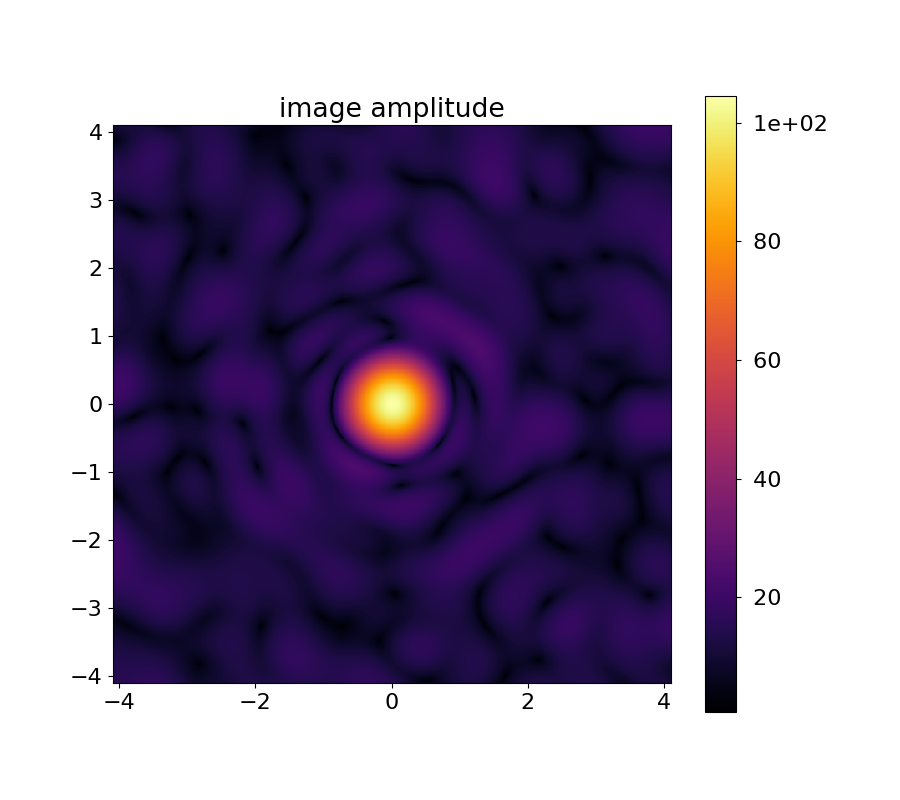
\includegraphics[width=\textwidth]{pictures/error_pics/errors2out_abs.png}
        \end{minipage}
        \caption{$\sigma_{\eps} = \pi/6 \qq*{,} l_c = \SI{0.1}{m}$}\label{fig:corrpic:1}
    \end{subfigure}%
    \hfill
    \begin{subfigure}{0.5\textwidth}
        \begin{minipage}{0.5\textwidth}
            \centering
            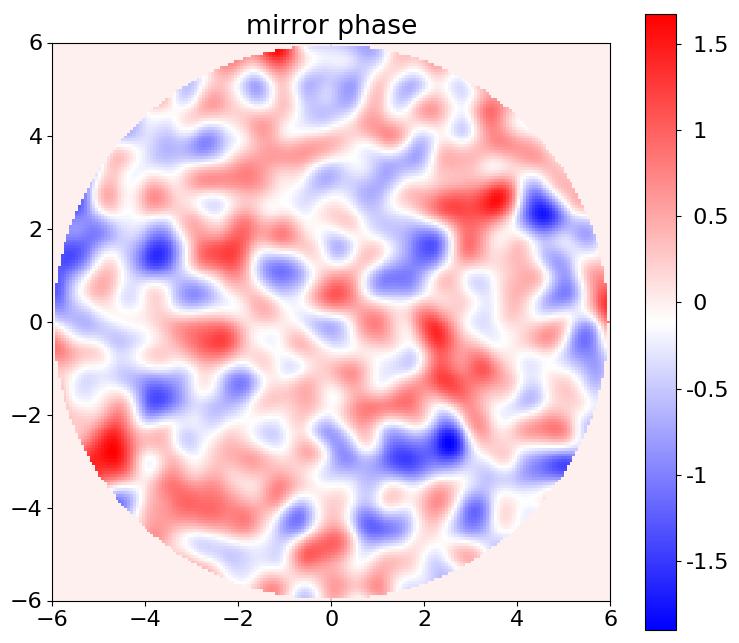
\includegraphics[width=\textwidth]{pictures/error_pics/errors3in_phase.png}
        \end{minipage}%
        \begin{minipage}{0.5\textwidth}
            \centering
            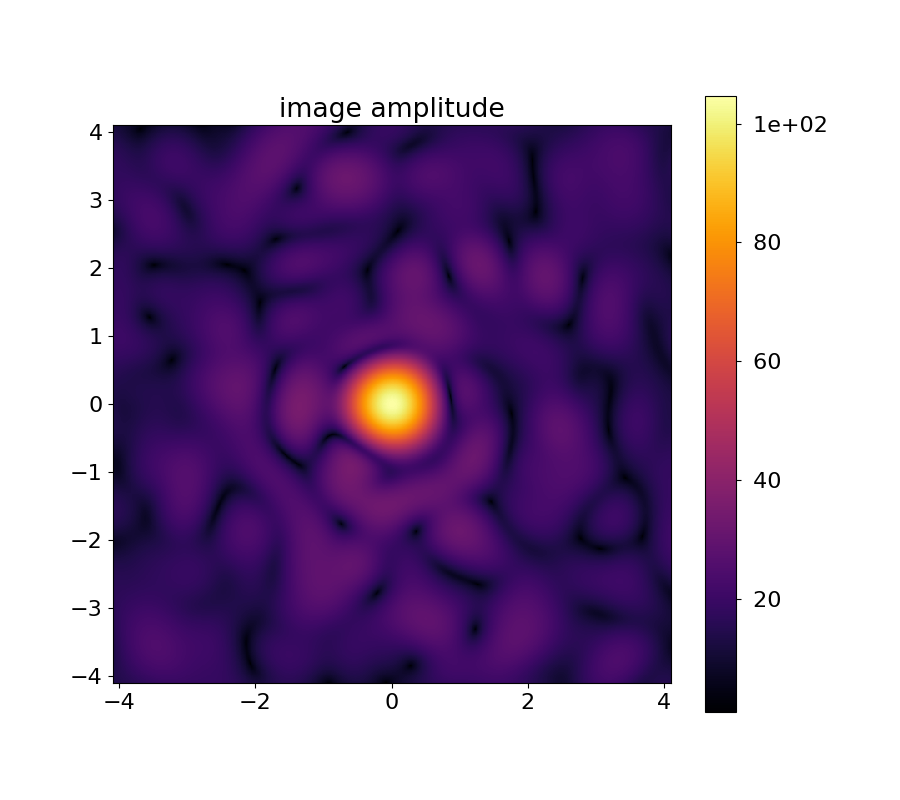
\includegraphics[width=\textwidth]{pictures/error_pics/errors3out_abs.png}
        \end{minipage}
        \caption{$\sigma_{\eps} = \pi/6 \qq*{,} l_c = \SI{0.3}{m}$}\label{fig:corrpic:2}
    \end{subfigure}

    \begin{subfigure}{0.5\textwidth}
        \begin{minipage}{0.5\textwidth}
            \centering
            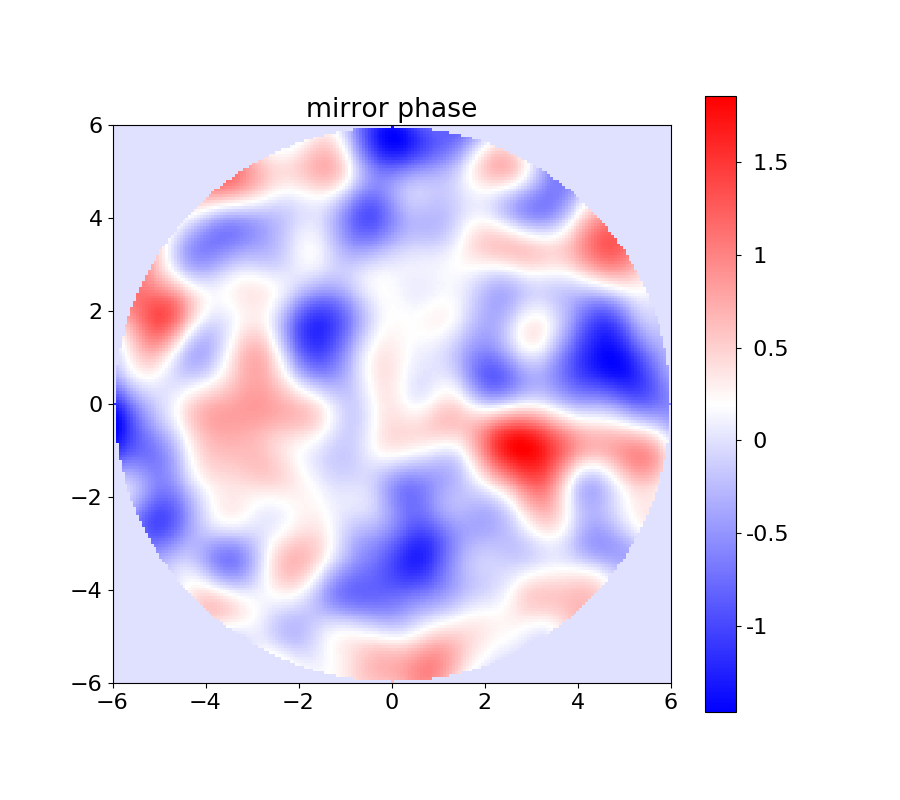
\includegraphics[width=\textwidth]{pictures/error_pics/errors4in_phase.png}
        \end{minipage}%
        \begin{minipage}{0.5\textwidth}
            \centering
            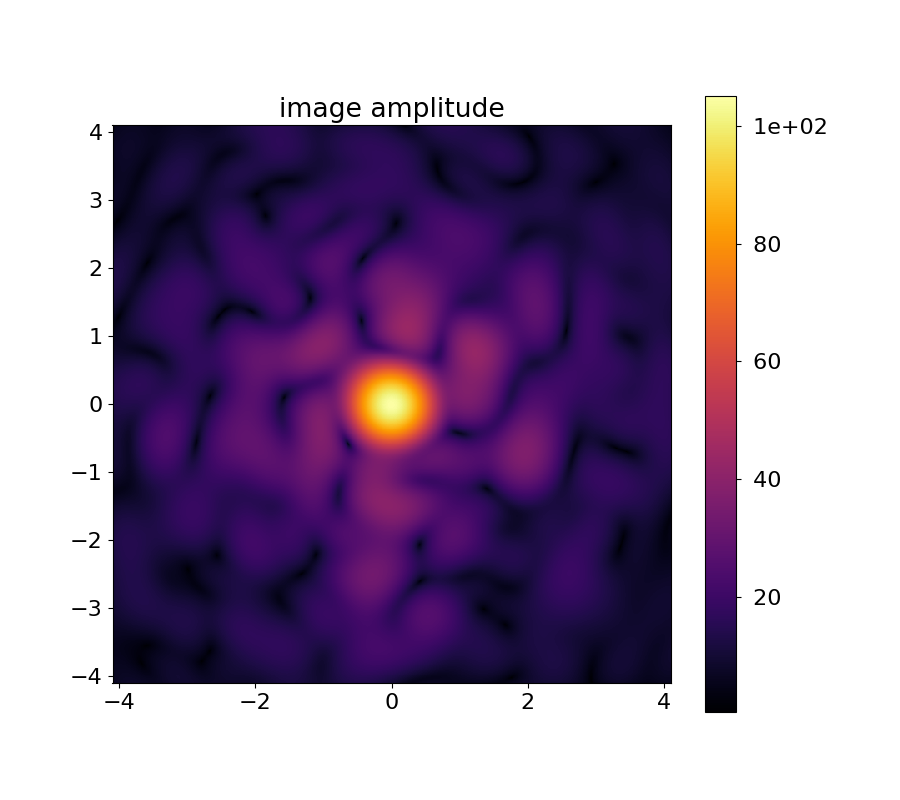
\includegraphics[width=\textwidth]{pictures/error_pics/errors4out_abs.png}
        \end{minipage}
        \caption{$\sigma_{\eps} = \pi/6 \qq*{,} l_c = \SI{0.5}{m}$}\label{fig:corrpic:3}
    \end{subfigure}%
    \hfill
    \begin{subfigure}{0.5\textwidth}
        \begin{minipage}{0.5\textwidth}
            \centering
            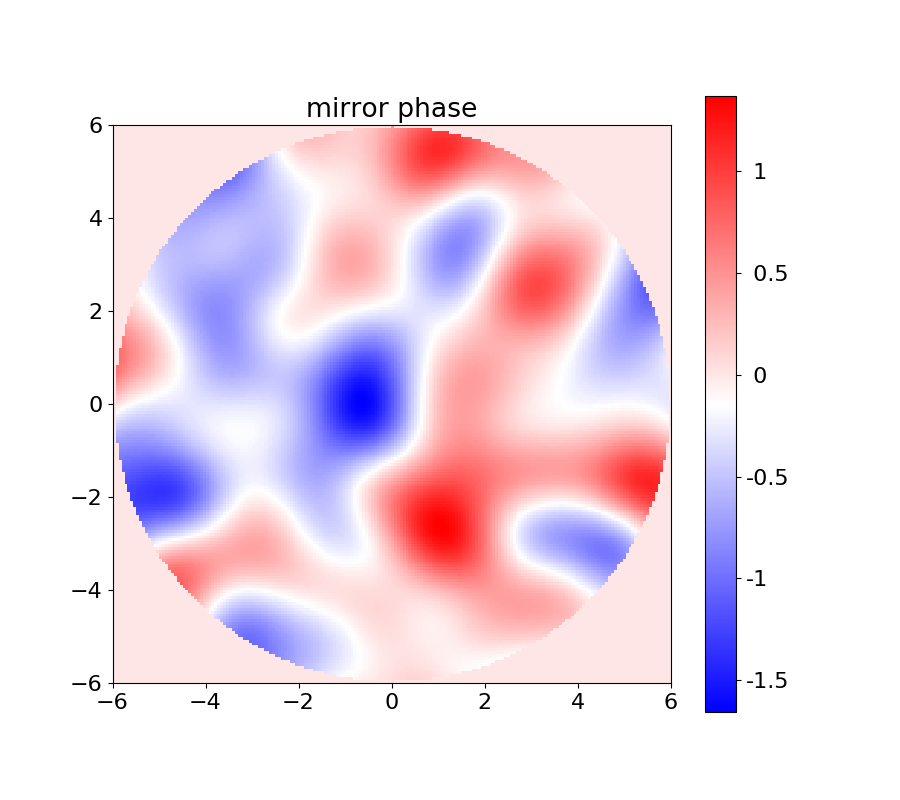
\includegraphics[width=\textwidth]{pictures/error_pics/errors5in_phase.png}
        \end{minipage}%
        \begin{minipage}{0.5\textwidth}
            \centering
            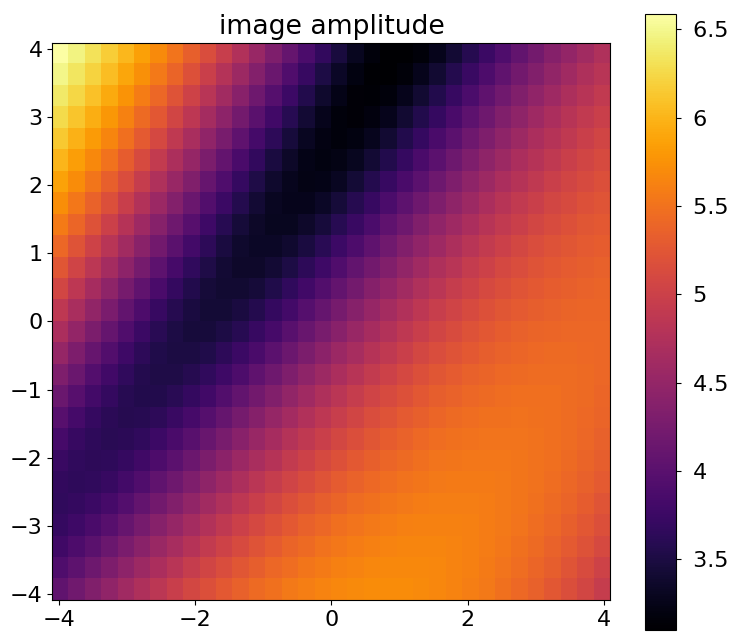
\includegraphics[width=\textwidth]{pictures/error_pics/errors5out_abs.png}
        \end{minipage}
        \caption{$\sigma_{\eps} = \pi/6 \qq*{,} l_c = \SI{0.8}{m}$}\label{fig:corrpic:4}
    \end{subfigure}

    \caption{Typical correlated error aperture functions and resulting diffraction patterns. Amplitudes are raised to the power $1/2$ to make features easier to see. Note that at larger correlation length, the central peak is absent.}\label{fig:corrpic}
\end{figure}
\restoregeometry{}

\section{Conclusion}\label{sec:conclusion}
I performed a computational study of the effects of wavefront error, such as those produced by deviations from the parabolic shape, on the images produced by telescope mirrors. A program was written in \CC{} to calculate the far-field diffraction pattern of a general mirror shape using a Fast Fourier Transform algorithm. It was tested with known mirror shapes and found to perform as expected.

The effect of gaussian-tapered illumination on the diffraction pattern was investigated. It was found to slightly widen the central maximum and decrease the peak intensity, but greatly reduce the sharpness of secondary rings found in a typical Airy pattern. A central hole, such as the one due to a secondary mirror, was found to have minimal effects on the beam.

The effects of two types of wavefront error were studied: random and spatially correlated. In both cases, an increase in the typical depth of the defects, i.e.\ the RMS phase error, was found to decrease the central amplitude of the diffraction pattern, thus decreasing the apparent brightness of objects seen through the telescope.

The spatial distribution of errors was seen to affect the spatial distribution of fluctuations in the image, but not its brightness or the width of the central maximum. For wider deformations, the fluctuations were concentrated closer to the central peak, whereas for denser and smaller deformations the fluctuations were spread out farther in the image plane. Thus, small and dense deformations have worse effects on the telescope's resolution.

\paragraph{Word count:} \textbf{2949}

\printbibliography{}
\pagebreak

\appendix
\newgeometry{top=1cm,left=1cm,right=1cm}
\section{Code listing}
\subsection{Numerical routines in C++}

\subsubsection{src/cpp/main.cpp}
\inputminted[fontsize=\footnotesize]{C++}{../src/cpp/main.cpp}

\subsubsection{src/cpp/util.h}
\inputminted[fontsize=\footnotesize]{C++}{../src/cpp/util.h}

\subsubsection{src/cpp/util.cpp}
\inputminted[fontsize=\footnotesize]{C++}{../src/cpp/util.cpp}

\subsubsection{src/cpp/array2d.h}
\inputminted[fontsize=\footnotesize]{C++}{../src/cpp/array2d.h}

\subsubsection{src/cpp/array2d.cpp}
\inputminted[fontsize=\footnotesize]{C++}{../src/cpp/array2d.cpp}

\subsubsection{src/cpp/generators.cpp}
\inputminted[fontsize=\footnotesize]{C++}{../src/cpp/generators.cpp}

\subsection{Plotting in Python}

\subsubsection{src/scripts/util.py}
\inputminted[fontsize=\footnotesize]{Python}{../src/scripts/util.py}

\subsubsection{src/scripts/write\_config.py}
\inputminted[fontsize=\footnotesize]{Python}{../src/scripts/write_config.py}

\subsubsection{src/scripts/make\_pictures.py}
\inputminted[fontsize=\footnotesize]{Python}{../src/scripts/make_pictures.py}

\subsubsection{src/scripts/tests.py}
\inputminted[fontsize=\footnotesize]{Python}{../src/scripts/tests.py}

\subsubsection{src/scripts/gauss.py}
\inputminted[fontsize=\footnotesize]{Python}{../src/scripts/gauss.py}

\subsubsection{src/scripts/hole.py}
\inputminted[fontsize=\footnotesize]{Python}{../src/scripts/hole.py}

\subsubsection{src/scripts/rand.py}
\inputminted[fontsize=\footnotesize]{Python}{../src/scripts/rand.py}

\subsubsection{src/scripts/rms\_test.py}
\inputminted[fontsize=\footnotesize]{Python}{../src/scripts/rms_test.py}

\subsubsection{src/scripts/corr.py}
\inputminted[fontsize=\footnotesize]{Python}{../src/scripts/corr.py}

\restoregeometry{}

\end{document}